Le misure sono state effettuate sull'amplificatore non invertente utilizzato al punto precedente e applicando una tensione sinusoidale 
di frequenza variabile mantenendo l'ampiezza $V_s= 2 V_{pp}$.

\subsection{Amplificatore con A=10}
Le resistenze inserite sono le stesse dello schema precedente, e quindi anche l'amplificazione teorica.

\begin{grafico}
 \centering 
 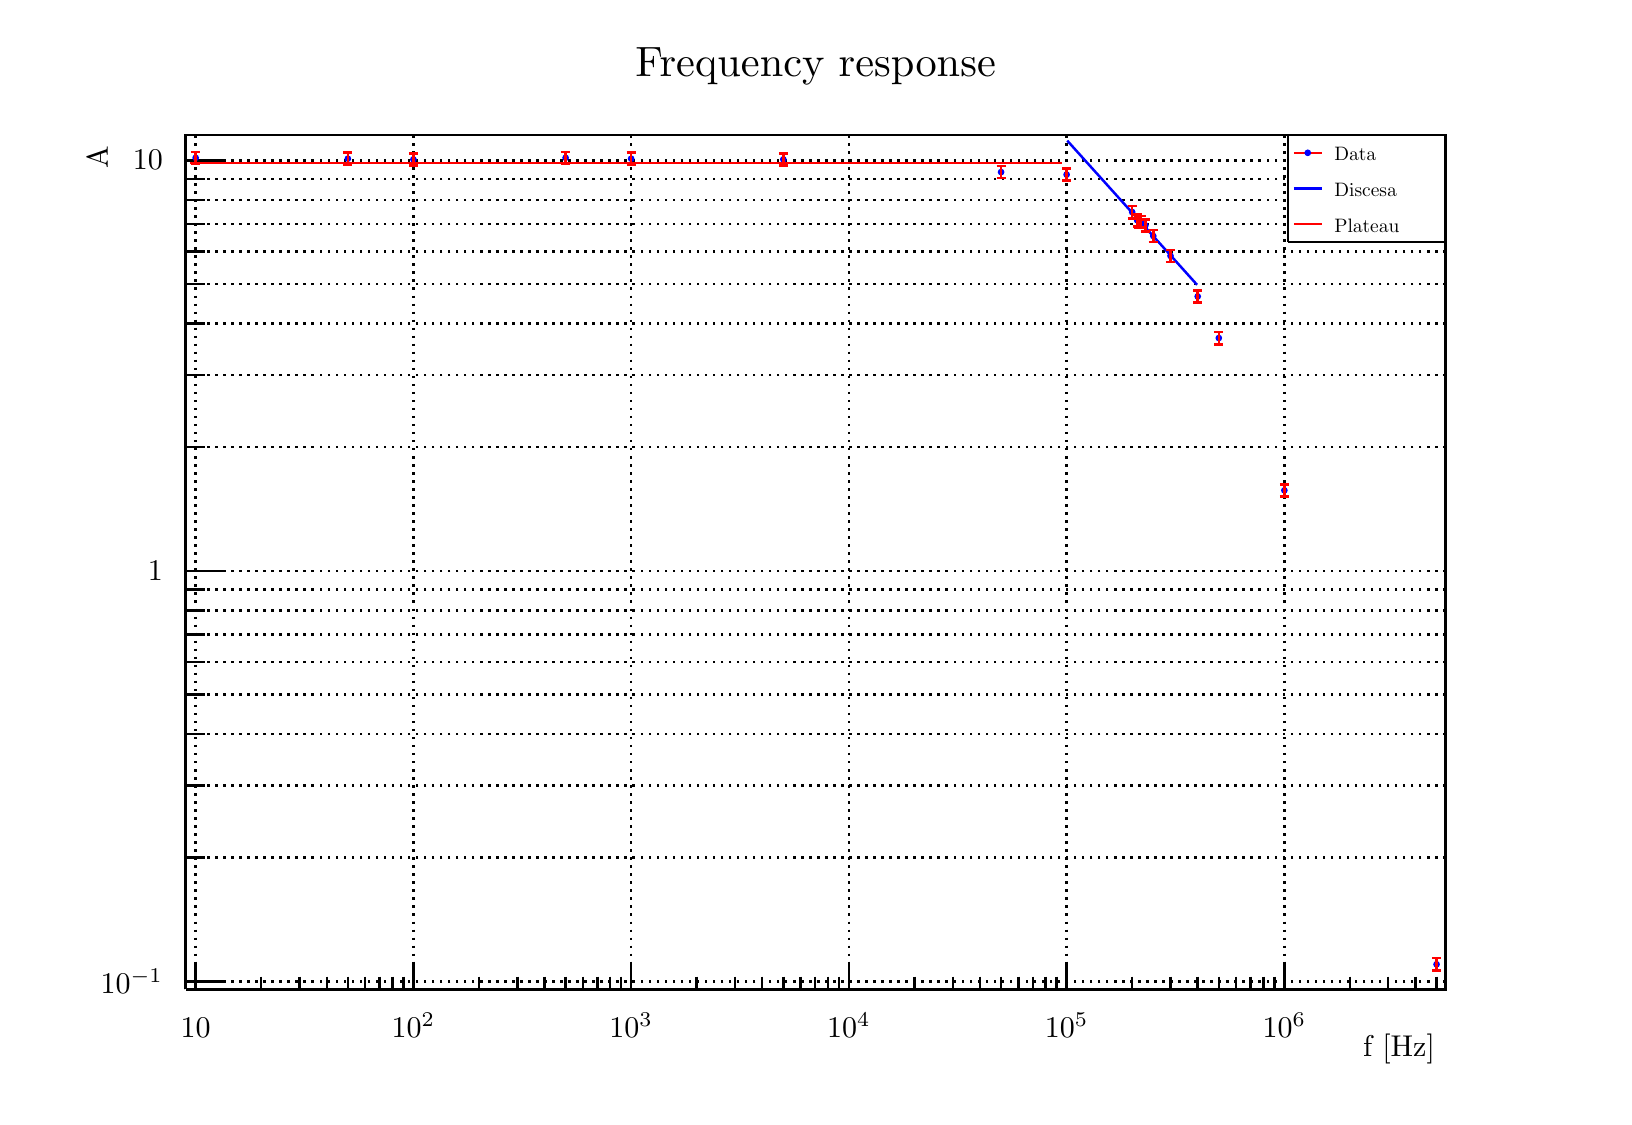
\begin{tikzpicture}
\pgfdeclareplotmark{cross} {
\pgfpathmoveto{\pgfpoint{-0.3\pgfplotmarksize}{\pgfplotmarksize}}
\pgfpathlineto{\pgfpoint{+0.3\pgfplotmarksize}{\pgfplotmarksize}}
\pgfpathlineto{\pgfpoint{+0.3\pgfplotmarksize}{0.3\pgfplotmarksize}}
\pgfpathlineto{\pgfpoint{+1\pgfplotmarksize}{0.3\pgfplotmarksize}}
\pgfpathlineto{\pgfpoint{+1\pgfplotmarksize}{-0.3\pgfplotmarksize}}
\pgfpathlineto{\pgfpoint{+0.3\pgfplotmarksize}{-0.3\pgfplotmarksize}}
\pgfpathlineto{\pgfpoint{+0.3\pgfplotmarksize}{-1.\pgfplotmarksize}}
\pgfpathlineto{\pgfpoint{-0.3\pgfplotmarksize}{-1.\pgfplotmarksize}}
\pgfpathlineto{\pgfpoint{-0.3\pgfplotmarksize}{-0.3\pgfplotmarksize}}
\pgfpathlineto{\pgfpoint{-1.\pgfplotmarksize}{-0.3\pgfplotmarksize}}
\pgfpathlineto{\pgfpoint{-1.\pgfplotmarksize}{0.3\pgfplotmarksize}}
\pgfpathlineto{\pgfpoint{-0.3\pgfplotmarksize}{0.3\pgfplotmarksize}}
\pgfpathclose
\pgfusepathqstroke
}
\pgfdeclareplotmark{cross*} {
\pgfpathmoveto{\pgfpoint{-0.3\pgfplotmarksize}{\pgfplotmarksize}}
\pgfpathlineto{\pgfpoint{+0.3\pgfplotmarksize}{\pgfplotmarksize}}
\pgfpathlineto{\pgfpoint{+0.3\pgfplotmarksize}{0.3\pgfplotmarksize}}
\pgfpathlineto{\pgfpoint{+1\pgfplotmarksize}{0.3\pgfplotmarksize}}
\pgfpathlineto{\pgfpoint{+1\pgfplotmarksize}{-0.3\pgfplotmarksize}}
\pgfpathlineto{\pgfpoint{+0.3\pgfplotmarksize}{-0.3\pgfplotmarksize}}
\pgfpathlineto{\pgfpoint{+0.3\pgfplotmarksize}{-1.\pgfplotmarksize}}
\pgfpathlineto{\pgfpoint{-0.3\pgfplotmarksize}{-1.\pgfplotmarksize}}
\pgfpathlineto{\pgfpoint{-0.3\pgfplotmarksize}{-0.3\pgfplotmarksize}}
\pgfpathlineto{\pgfpoint{-1.\pgfplotmarksize}{-0.3\pgfplotmarksize}}
\pgfpathlineto{\pgfpoint{-1.\pgfplotmarksize}{0.3\pgfplotmarksize}}
\pgfpathlineto{\pgfpoint{-0.3\pgfplotmarksize}{0.3\pgfplotmarksize}}
\pgfpathclose
\pgfusepathqfillstroke
}
\pgfdeclareplotmark{newstar} {
\pgfpathmoveto{\pgfqpoint{0pt}{\pgfplotmarksize}}
\pgfpathlineto{\pgfqpointpolar{44}{0.5\pgfplotmarksize}}
\pgfpathlineto{\pgfqpointpolar{18}{\pgfplotmarksize}}
\pgfpathlineto{\pgfqpointpolar{-20}{0.5\pgfplotmarksize}}
\pgfpathlineto{\pgfqpointpolar{-54}{\pgfplotmarksize}}
\pgfpathlineto{\pgfqpointpolar{-90}{0.5\pgfplotmarksize}}
\pgfpathlineto{\pgfqpointpolar{234}{\pgfplotmarksize}}
\pgfpathlineto{\pgfqpointpolar{198}{0.5\pgfplotmarksize}}
\pgfpathlineto{\pgfqpointpolar{162}{\pgfplotmarksize}}
\pgfpathlineto{\pgfqpointpolar{134}{0.5\pgfplotmarksize}}
\pgfpathclose
\pgfusepathqstroke
}
\pgfdeclareplotmark{newstar*} {
\pgfpathmoveto{\pgfqpoint{0pt}{\pgfplotmarksize}}
\pgfpathlineto{\pgfqpointpolar{44}{0.5\pgfplotmarksize}}
\pgfpathlineto{\pgfqpointpolar{18}{\pgfplotmarksize}}
\pgfpathlineto{\pgfqpointpolar{-20}{0.5\pgfplotmarksize}}
\pgfpathlineto{\pgfqpointpolar{-54}{\pgfplotmarksize}}
\pgfpathlineto{\pgfqpointpolar{-90}{0.5\pgfplotmarksize}}
\pgfpathlineto{\pgfqpointpolar{234}{\pgfplotmarksize}}
\pgfpathlineto{\pgfqpointpolar{198}{0.5\pgfplotmarksize}}
\pgfpathlineto{\pgfqpointpolar{162}{\pgfplotmarksize}}
\pgfpathlineto{\pgfqpointpolar{134}{0.5\pgfplotmarksize}}
\pgfpathclose
\pgfusepathqfillstroke
}
\definecolor{c}{rgb}{1,1,1};
\draw [color=c, fill=c] (0,0) rectangle (20,13.5632);
\draw [color=c, fill=c] (2,1.35632) rectangle (18,12.2069);
\definecolor{c}{rgb}{0,0,0};
\draw [c,line width=0.9] (2,1.35632) -- (2,12.2069) -- (18,12.2069) -- (18,1.35632) -- (2,1.35632);
\definecolor{c}{rgb}{1,1,1};
\draw [color=c, fill=c] (2,1.35632) rectangle (18,12.2069);
\definecolor{c}{rgb}{0,0,0};
\draw [c,line width=0.9] (2,1.35632) -- (2,12.2069) -- (18,12.2069) -- (18,1.35632) -- (2,1.35632);
\draw [c,line width=0.9] (2,1.35632) -- (18,1.35632);
\draw [c,dotted,line width=0.9] (2.12653,12.2069) -- (2.12653,1.35632);
\draw [c,dotted,line width=0.9] (4.89177,12.2069) -- (4.89177,1.35632);
\draw [c,dotted,line width=0.9] (7.657,12.2069) -- (7.657,1.35632);
\draw [c,dotted,line width=0.9] (10.4222,12.2069) -- (10.4222,1.35632);
\draw [c,dotted,line width=0.9] (13.1875,12.2069) -- (13.1875,1.35632);
\draw [c,dotted,line width=0.9] (15.9527,12.2069) -- (15.9527,1.35632);
\draw [c,line width=0.9] (2,1.35632) -- (2,12.2069);
\draw [c,dotted,line width=0.9] (18,1.4593) -- (2,1.4593);
\draw [c,dotted,line width=0.9] (18,3.02864) -- (2,3.02864);
\draw [c,dotted,line width=0.9] (18,3.94665) -- (2,3.94665);
\draw [c,dotted,line width=0.9] (18,4.59799) -- (2,4.59799);
\draw [c,dotted,line width=0.9] (18,5.1032) -- (2,5.1032);
\draw [c,dotted,line width=0.9] (18,5.516) -- (2,5.516);
\draw [c,dotted,line width=0.9] (18,5.86501) -- (2,5.86501);
\draw [c,dotted,line width=0.9] (18,6.16733) -- (2,6.16733);
\draw [c,dotted,line width=0.9] (18,6.434) -- (2,6.434);
\draw [c,dotted,line width=0.9] (18,6.67255) -- (2,6.67255);
\draw [c,dotted,line width=0.9] (18,8.24189) -- (2,8.24189);
\draw [c,dotted,line width=0.9] (18,9.1599) -- (2,9.1599);
\draw [c,dotted,line width=0.9] (18,9.81124) -- (2,9.81124);
\draw [c,dotted,line width=0.9] (18,10.3165) -- (2,10.3165);
\draw [c,dotted,line width=0.9] (18,10.7292) -- (2,10.7292);
\draw [c,dotted,line width=0.9] (18,11.0783) -- (2,11.0783);
\draw [c,dotted,line width=0.9] (18,11.3806) -- (2,11.3806);
\draw [c,dotted,line width=0.9] (18,11.6472) -- (2,11.6472);
\draw [c,dotted,line width=0.9] (18,11.8858) -- (2,11.8858);
\draw [c,line width=0.9] (2,1.35632) -- (18,1.35632);
\draw [anchor= east] (18,0.596782) node[scale=1.08496, color=c, rotate=0]{f [Hz]};
\draw [c,line width=0.9] (2.12653,1.68184) -- (2.12653,1.35632);
\draw [anchor=base] (2.12653,0.742586) node[scale=1.08496, color=c, rotate=0]{10};
\draw [c,line width=0.9] (2.95895,1.51908) -- (2.95895,1.35632);
\draw [c,line width=0.9] (3.44588,1.51908) -- (3.44588,1.35632);
\draw [c,line width=0.9] (3.79137,1.51908) -- (3.79137,1.35632);
\draw [c,line width=0.9] (4.05935,1.51908) -- (4.05935,1.35632);
\draw [c,line width=0.9] (4.2783,1.51908) -- (4.2783,1.35632);
\draw [c,line width=0.9] (4.46343,1.51908) -- (4.46343,1.35632);
\draw [c,line width=0.9] (4.62379,1.51908) -- (4.62379,1.35632);
\draw [c,line width=0.9] (4.76524,1.51908) -- (4.76524,1.35632);
\draw [c,line width=0.9] (4.89177,1.68184) -- (4.89177,1.35632);
\draw [anchor=base] (4.89177,0.742586) node[scale=1.08496, color=c, rotate=0]{$10^{2}$};
\draw [c,line width=0.9] (5.72419,1.51908) -- (5.72419,1.35632);
\draw [c,line width=0.9] (6.21112,1.51908) -- (6.21112,1.35632);
\draw [c,line width=0.9] (6.55661,1.51908) -- (6.55661,1.35632);
\draw [c,line width=0.9] (6.82458,1.51908) -- (6.82458,1.35632);
\draw [c,line width=0.9] (7.04354,1.51908) -- (7.04354,1.35632);
\draw [c,line width=0.9] (7.22866,1.51908) -- (7.22866,1.35632);
\draw [c,line width=0.9] (7.38903,1.51908) -- (7.38903,1.35632);
\draw [c,line width=0.9] (7.53047,1.51908) -- (7.53047,1.35632);
\draw [c,line width=0.9] (7.657,1.68184) -- (7.657,1.35632);
\draw [anchor=base] (7.657,0.742586) node[scale=1.08496, color=c, rotate=0]{$10^{3}$};
\draw [c,line width=0.9] (8.48942,1.51908) -- (8.48942,1.35632);
\draw [c,line width=0.9] (8.97636,1.51908) -- (8.97636,1.35632);
\draw [c,line width=0.9] (9.32184,1.51908) -- (9.32184,1.35632);
\draw [c,line width=0.9] (9.58982,1.51908) -- (9.58982,1.35632);
\draw [c,line width=0.9] (9.80878,1.51908) -- (9.80878,1.35632);
\draw [c,line width=0.9] (9.9939,1.51908) -- (9.9939,1.35632);
\draw [c,line width=0.9] (10.1543,1.51908) -- (10.1543,1.35632);
\draw [c,line width=0.9] (10.2957,1.51908) -- (10.2957,1.35632);
\draw [c,line width=0.9] (10.4222,1.68184) -- (10.4222,1.35632);
\draw [anchor=base] (10.4222,0.742586) node[scale=1.08496, color=c, rotate=0]{$10^{4}$};
\draw [c,line width=0.9] (11.2547,1.51908) -- (11.2547,1.35632);
\draw [c,line width=0.9] (11.7416,1.51908) -- (11.7416,1.35632);
\draw [c,line width=0.9] (12.0871,1.51908) -- (12.0871,1.35632);
\draw [c,line width=0.9] (12.3551,1.51908) -- (12.3551,1.35632);
\draw [c,line width=0.9] (12.574,1.51908) -- (12.574,1.35632);
\draw [c,line width=0.9] (12.7591,1.51908) -- (12.7591,1.35632);
\draw [c,line width=0.9] (12.9195,1.51908) -- (12.9195,1.35632);
\draw [c,line width=0.9] (13.061,1.51908) -- (13.061,1.35632);
\draw [c,line width=0.9] (13.1875,1.68184) -- (13.1875,1.35632);
\draw [anchor=base] (13.1875,0.742586) node[scale=1.08496, color=c, rotate=0]{$10^{5}$};
\draw [c,line width=0.9] (14.0199,1.51908) -- (14.0199,1.35632);
\draw [c,line width=0.9] (14.5068,1.51908) -- (14.5068,1.35632);
\draw [c,line width=0.9] (14.8523,1.51908) -- (14.8523,1.35632);
\draw [c,line width=0.9] (15.1203,1.51908) -- (15.1203,1.35632);
\draw [c,line width=0.9] (15.3393,1.51908) -- (15.3393,1.35632);
\draw [c,line width=0.9] (15.5244,1.51908) -- (15.5244,1.35632);
\draw [c,line width=0.9] (15.6847,1.51908) -- (15.6847,1.35632);
\draw [c,line width=0.9] (15.8262,1.51908) -- (15.8262,1.35632);
\draw [c,line width=0.9] (15.9527,1.68184) -- (15.9527,1.35632);
\draw [anchor=base] (15.9527,0.742586) node[scale=1.08496, color=c, rotate=0]{$10^{6}$};
\draw [c,line width=0.9] (16.7851,1.51908) -- (16.7851,1.35632);
\draw [c,line width=0.9] (17.2721,1.51908) -- (17.2721,1.35632);
\draw [c,line width=0.9] (17.6176,1.51908) -- (17.6176,1.35632);
\draw [c,line width=0.9] (17.8855,1.51908) -- (17.8855,1.35632);
\draw [c,line width=0.9] (2,1.35632) -- (2,12.2069);
\draw [anchor= east] (0.88,12.2069) node[scale=1.08496, color=c, rotate=90]{A};
\draw [c,line width=0.9] (2.48,1.4593) -- (2,1.4593);
\draw [anchor= east] (1.844,1.4593) node[scale=1.08496, color=c, rotate=0]{$10^{-1}$};
\draw [c,line width=0.9] (2.24,3.02864) -- (2,3.02864);
\draw [c,line width=0.9] (2.24,3.94665) -- (2,3.94665);
\draw [c,line width=0.9] (2.24,4.59799) -- (2,4.59799);
\draw [c,line width=0.9] (2.24,5.1032) -- (2,5.1032);
\draw [c,line width=0.9] (2.24,5.516) -- (2,5.516);
\draw [c,line width=0.9] (2.24,5.86501) -- (2,5.86501);
\draw [c,line width=0.9] (2.24,6.16733) -- (2,6.16733);
\draw [c,line width=0.9] (2.24,6.434) -- (2,6.434);
\draw [c,line width=0.9] (2.48,6.67255) -- (2,6.67255);
\draw [anchor= east] (1.844,6.67255) node[scale=1.08496, color=c, rotate=0]{1};
\draw [c,line width=0.9] (2.24,8.24189) -- (2,8.24189);
\draw [c,line width=0.9] (2.24,9.1599) -- (2,9.1599);
\draw [c,line width=0.9] (2.24,9.81124) -- (2,9.81124);
\draw [c,line width=0.9] (2.24,10.3165) -- (2,10.3165);
\draw [c,line width=0.9] (2.24,10.7292) -- (2,10.7292);
\draw [c,line width=0.9] (2.24,11.0783) -- (2,11.0783);
\draw [c,line width=0.9] (2.24,11.3806) -- (2,11.3806);
\draw [c,line width=0.9] (2.24,11.6472) -- (2,11.6472);
\draw [c,line width=0.9] (2.48,11.8858) -- (2,11.8858);
\draw [anchor= east] (1.844,11.8858) node[scale=1.08496, color=c, rotate=0]{10};
\definecolor{c}{rgb}{0,0,1};
\foreach \P in {(2.12653,11.9173), (4.05935,11.9061), (4.89177,11.8971), (6.82459,11.9173), (7.65701,11.9061), (9.58983,11.8971), (12.3551,11.736), (13.1875,11.7044), (14.0199,11.2284), (14.0842,11.1231), (14.1068,11.1072), (14.1344,11.1072),
 (14.1877,11.0588), (14.2879,10.9244), (14.5068,10.6719), (14.8523,10.157), (15.1203,9.6286), (15.9527,7.69382), (17.8855,1.67509)}{\draw[mark options={color=c,fill=c},mark size=1.681682pt,mark=*,mark size=1pt] plot coordinates {\P};}
\definecolor{c}{rgb}{1,0,0};
\draw [c,line width=0.9] (2.05724,11.8539) -- (2.16911,11.8539) -- (2.28099,11.8539) -- (2.39286,11.8539) -- (2.50474,11.8539) -- (2.61661,11.8539) -- (2.72849,11.8539) -- (2.84036,11.8539) -- (2.95224,11.8539) -- (3.06411,11.8539) --
 (3.17599,11.8539) -- (3.28786,11.8539) -- (3.39974,11.8539) -- (3.51161,11.8539) -- (3.62349,11.8539) -- (3.73536,11.8539) -- (3.84724,11.8539) -- (3.95911,11.8539) -- (4.07099,11.8539) -- (4.18286,11.8539) -- (4.29474,11.8539) -- (4.40661,11.8539)
 -- (4.51849,11.8539) -- (4.63036,11.8539) -- (4.74224,11.8539) -- (4.85411,11.8539) -- (4.96599,11.8539) -- (5.07786,11.8539) -- (5.18974,11.8539) -- (5.30161,11.8539) -- (5.41349,11.8539) -- (5.52536,11.8539) -- (5.63724,11.8539) --
 (5.74911,11.8539) -- (5.86099,11.8539) -- (5.97286,11.8539) -- (6.08474,11.8539) -- (6.19661,11.8539) -- (6.30849,11.8539) -- (6.42036,11.8539) -- (6.53224,11.8539) -- (6.64411,11.8539) -- (6.75599,11.8539) -- (6.86786,11.8539) -- (6.97974,11.8539)
 -- (7.09161,11.8539) -- (7.20349,11.8539) -- (7.31536,11.8539) -- (7.42724,11.8539) -- (7.53911,11.8539);
\draw [c,line width=0.9] (7.53911,11.8539) -- (7.65099,11.8539) -- (7.76286,11.8539) -- (7.87474,11.8539) -- (7.98661,11.8539) -- (8.09849,11.8539) -- (8.21036,11.8539) -- (8.32224,11.8539) -- (8.43411,11.8539) -- (8.54599,11.8539) --
 (8.65786,11.8539) -- (8.76974,11.8539) -- (8.88161,11.8539) -- (8.99349,11.8539) -- (9.10536,11.8539) -- (9.21724,11.8539) -- (9.32911,11.8539) -- (9.44099,11.8539) -- (9.55286,11.8539) -- (9.66474,11.8539) -- (9.77661,11.8539) -- (9.88849,11.8539)
 -- (10.0004,11.8539) -- (10.1122,11.8539) -- (10.2241,11.8539) -- (10.336,11.8539) -- (10.4479,11.8539) -- (10.5597,11.8539) -- (10.6716,11.8539) -- (10.7835,11.8539) -- (10.8954,11.8539) -- (11.0072,11.8539) -- (11.1191,11.8539) -- (11.231,11.8539)
 -- (11.3429,11.8539) -- (11.4547,11.8539) -- (11.5666,11.8539) -- (11.6785,11.8539) -- (11.7904,11.8539) -- (11.9022,11.8539) -- (12.0141,11.8539) -- (12.126,11.8539) -- (12.2379,11.8539) -- (12.3497,11.8539) -- (12.4616,11.8539) --
 (12.5735,11.8539) -- (12.6854,11.8539) -- (12.7972,11.8539) -- (12.9091,11.8539) -- (13.021,11.8539);
\draw [c,line width=0.9] (13.021,11.8539) -- (13.1329,11.8539);
\definecolor{c}{rgb}{0,0,1};
\draw [c,line width=0.9] (13.1958,12.1351) -- (13.2125,12.1166) -- (13.2291,12.0981) -- (13.2458,12.0796) -- (13.2624,12.0611) -- (13.2791,12.0427) -- (13.2957,12.0242) -- (13.3124,12.0057) -- (13.329,11.9872) -- (13.3457,11.9687) --
 (13.3623,11.9502) -- (13.379,11.9317) -- (13.3956,11.9132) -- (13.4123,11.8947) -- (13.4289,11.8762) -- (13.4456,11.8577) -- (13.4622,11.8393) -- (13.4789,11.8208) -- (13.4955,11.8023) -- (13.5122,11.7838) -- (13.5288,11.7653) -- (13.5455,11.7468)
 -- (13.5621,11.7283) -- (13.5788,11.7098) -- (13.5954,11.6913) -- (13.6121,11.6728) -- (13.6287,11.6544) -- (13.6454,11.6359) -- (13.662,11.6174) -- (13.6786,11.5989) -- (13.6953,11.5804) -- (13.7119,11.5619) -- (13.7286,11.5434) --
 (13.7452,11.5249) -- (13.7619,11.5064) -- (13.7785,11.4879) -- (13.7952,11.4694) -- (13.8118,11.451) -- (13.8285,11.4325) -- (13.8451,11.414) -- (13.8618,11.3955) -- (13.8784,11.377) -- (13.8951,11.3585) -- (13.9117,11.34) -- (13.9284,11.3215) --
 (13.945,11.303) -- (13.9617,11.2845) -- (13.9783,11.266) -- (13.995,11.2476) -- (14.0116,11.2291);
\draw [c,line width=0.9] (14.0116,11.2291) -- (14.0283,11.2106) -- (14.0449,11.1921) -- (14.0616,11.1736) -- (14.0782,11.1551) -- (14.0949,11.1366) -- (14.1115,11.1181) -- (14.1281,11.0996) -- (14.1448,11.0811) -- (14.1614,11.0627) --
 (14.1781,11.0442) -- (14.1947,11.0257) -- (14.2114,11.0072) -- (14.228,10.9887) -- (14.2447,10.9702) -- (14.2613,10.9517) -- (14.278,10.9332) -- (14.2946,10.9147) -- (14.3113,10.8962) -- (14.3279,10.8777) -- (14.3446,10.8593) -- (14.3612,10.8408) --
 (14.3779,10.8223) -- (14.3945,10.8038) -- (14.4112,10.7853) -- (14.4278,10.7668) -- (14.4445,10.7483) -- (14.4611,10.7298) -- (14.4778,10.7113) -- (14.4944,10.6928) -- (14.5111,10.6744) -- (14.5277,10.6559) -- (14.5444,10.6374) -- (14.561,10.6189)
 -- (14.5777,10.6004) -- (14.5943,10.5819) -- (14.6109,10.5634) -- (14.6276,10.5449) -- (14.6442,10.5264) -- (14.6609,10.5079) -- (14.6775,10.4894) -- (14.6942,10.471) -- (14.7108,10.4525) -- (14.7275,10.434) -- (14.7441,10.4155) -- (14.7608,10.397)
 -- (14.7774,10.3785) -- (14.7941,10.36) -- (14.8107,10.3415) -- (14.8274,10.323);
\draw [c,line width=0.9] (14.8274,10.323) -- (14.844,10.3045);
\definecolor{c}{rgb}{1,0,0};
\draw [c,line width=0.9] (2.12653,11.9173) -- (2.12653,11.9932);
\draw [c,line width=0.9] (2.06906,11.9932) -- (2.184,11.9932);
\draw [c,line width=0.9] (2.12653,11.9173) -- (2.12653,11.8387);
\draw [c,line width=0.9] (2.06906,11.8387) -- (2.184,11.8387);
\draw [c,line width=0.9] (4.05935,11.9061) -- (4.05935,11.9821);
\draw [c,line width=0.9] (4.00188,11.9821) -- (4.11682,11.9821);
\draw [c,line width=0.9] (4.05935,11.9061) -- (4.05935,11.8275);
\draw [c,line width=0.9] (4.00188,11.8275) -- (4.11682,11.8275);
\draw [c,line width=0.9] (4.89177,11.8971) -- (4.89177,11.9731);
\draw [c,line width=0.9] (4.8343,11.9731) -- (4.94924,11.9731);
\draw [c,line width=0.9] (4.89177,11.8971) -- (4.89177,11.8184);
\draw [c,line width=0.9] (4.8343,11.8184) -- (4.94924,11.8184);
\draw [c,line width=0.9] (6.82459,11.9173) -- (6.82459,11.9932);
\draw [c,line width=0.9] (6.76712,11.9932) -- (6.88206,11.9932);
\draw [c,line width=0.9] (6.82459,11.9173) -- (6.82459,11.8387);
\draw [c,line width=0.9] (6.76712,11.8387) -- (6.88206,11.8387);
\draw [c,line width=0.9] (7.65701,11.9061) -- (7.65701,11.9821);
\draw [c,line width=0.9] (7.59954,11.9821) -- (7.71448,11.9821);
\draw [c,line width=0.9] (7.65701,11.9061) -- (7.65701,11.8275);
\draw [c,line width=0.9] (7.59954,11.8275) -- (7.71448,11.8275);
\draw [c,line width=0.9] (9.58983,11.8971) -- (9.58983,11.9731);
\draw [c,line width=0.9] (9.53235,11.9731) -- (9.6473,11.9731);
\draw [c,line width=0.9] (9.58983,11.8971) -- (9.58983,11.8184);
\draw [c,line width=0.9] (9.53235,11.8184) -- (9.6473,11.8184);
\draw [c,line width=0.9] (12.3551,11.736) -- (12.3551,11.8102);
\draw [c,line width=0.9] (12.2976,11.8102) -- (12.4125,11.8102);
\draw [c,line width=0.9] (12.3551,11.736) -- (12.3551,11.6594);
\draw [c,line width=0.9] (12.2976,11.6594) -- (12.4125,11.6594);
\draw [c,line width=0.9] (13.1875,11.7044) -- (13.1875,11.7787);
\draw [c,line width=0.9] (13.13,11.7787) -- (13.245,11.7787);
\draw [c,line width=0.9] (13.1875,11.7044) -- (13.1875,11.6276);
\draw [c,line width=0.9] (13.13,11.6276) -- (13.245,11.6276);
\draw [c,line width=0.9] (14.0199,11.2284) -- (14.0199,11.3056);
\draw [c,line width=0.9] (13.9624,11.3056) -- (14.0774,11.3056);
\draw [c,line width=0.9] (14.0199,11.2284) -- (14.0199,11.1485);
\draw [c,line width=0.9] (13.9624,11.1485) -- (14.0774,11.1485);
\draw [c,line width=0.9] (14.0842,11.1231) -- (14.0842,11.1971);
\draw [c,line width=0.9] (14.0267,11.1971) -- (14.1417,11.1971);
\draw [c,line width=0.9] (14.0842,11.1231) -- (14.0842,11.0466);
\draw [c,line width=0.9] (14.0267,11.0466) -- (14.1417,11.0466);
\draw [c,line width=0.9] (14.1068,11.1072) -- (14.1068,11.1812);
\draw [c,line width=0.9] (14.0493,11.1812) -- (14.1642,11.1812);
\draw [c,line width=0.9] (14.1068,11.1072) -- (14.1068,11.0306);
\draw [c,line width=0.9] (14.0493,11.0306) -- (14.1642,11.0306);
\draw [c,line width=0.9] (14.1344,11.1072) -- (14.1344,11.1812);
\draw [c,line width=0.9] (14.0769,11.1812) -- (14.1918,11.1812);
\draw [c,line width=0.9] (14.1344,11.1072) -- (14.1344,11.0306);
\draw [c,line width=0.9] (14.0769,11.0306) -- (14.1918,11.0306);
\draw [c,line width=0.9] (14.1877,11.0588) -- (14.1877,11.133);
\draw [c,line width=0.9] (14.1303,11.133) -- (14.2452,11.133);
\draw [c,line width=0.9] (14.1877,11.0588) -- (14.1877,10.982);
\draw [c,line width=0.9] (14.1303,10.982) -- (14.2452,10.982);
\draw [c,line width=0.9] (14.2879,10.9244) -- (14.2879,10.9993);
\draw [c,line width=0.9] (14.2304,10.9993) -- (14.3454,10.9993);
\draw [c,line width=0.9] (14.2879,10.9244) -- (14.2879,10.8468);
\draw [c,line width=0.9] (14.2304,10.8468) -- (14.3454,10.8468);
\draw [c,line width=0.9] (14.5068,10.6719) -- (14.5068,10.7484);
\draw [c,line width=0.9] (14.4494,10.7484) -- (14.5643,10.7484);
\draw [c,line width=0.9] (14.5068,10.6719) -- (14.5068,10.5928);
\draw [c,line width=0.9] (14.4494,10.5928) -- (14.5643,10.5928);
\draw [c,line width=0.9] (14.8523,10.157) -- (14.8523,10.2312);
\draw [c,line width=0.9] (14.7949,10.2312) -- (14.9098,10.2312);
\draw [c,line width=0.9] (14.8523,10.157) -- (14.8523,10.0803);
\draw [c,line width=0.9] (14.7949,10.0803) -- (14.9098,10.0803);
\draw [c,line width=0.9] (15.1203,9.6286) -- (15.1203,9.70596);
\draw [c,line width=0.9] (15.0628,9.70596) -- (15.1778,9.70596);
\draw [c,line width=0.9] (15.1203,9.6286) -- (15.1203,9.54849);
\draw [c,line width=0.9] (15.0628,9.54849) -- (15.1778,9.54849);
\draw [c,line width=0.9] (15.9527,7.69382) -- (15.9527,7.77021);
\draw [c,line width=0.9] (15.8952,7.77021) -- (16.0102,7.77021);
\draw [c,line width=0.9] (15.9527,7.69382) -- (15.9527,7.61476);
\draw [c,line width=0.9] (15.8952,7.61476) -- (16.0102,7.61476);
\draw [c,line width=0.9] (17.8855,1.67509) -- (17.8855,1.75256);
\draw [c,line width=0.9] (17.8281,1.75256) -- (17.943,1.75256);
\draw [c,line width=0.9] (17.8855,1.67509) -- (17.8855,1.59487);
\draw [c,line width=0.9] (17.8281,1.59487) -- (17.943,1.59487);
\definecolor{c}{rgb}{1,1,1};
\draw [color=c, fill=c] (16,10.8506) rectangle (18,12.2069);
\definecolor{c}{rgb}{0,0,0};
\draw [c,line width=0.9] (16,10.8506) -- (18,10.8506);
\draw [c,line width=0.9] (18,10.8506) -- (18,12.2069);
\draw [c,line width=0.9] (18,12.2069) -- (16,12.2069);
\draw [c,line width=0.9] (16,12.2069) -- (16,10.8506);
\draw [anchor=base west] (16.5,11.8791) node[scale=0.702031, color=c, rotate=0]{Data};
\definecolor{c}{rgb}{1,0,0};
\draw [c,line width=0.9] (16.075,11.9808) -- (16.425,11.9808);
\definecolor{c}{rgb}{0,0,1};
\foreach \P in {(16.25,11.9808)}{\draw[mark options={color=c,fill=c},mark size=1.681682pt,mark=*,mark size=1pt] plot coordinates {\P};}
\definecolor{c}{rgb}{0,0,0};
\draw [anchor=base west] (16.5,11.427) node[scale=0.702031, color=c, rotate=0]{Discesa};
\definecolor{c}{rgb}{0,0,1};
\draw [c,line width=0.9] (16.075,11.5287) -- (16.425,11.5287);
\definecolor{c}{rgb}{0,0,0};
\draw [anchor=base west] (16.5,10.9749) node[scale=0.702031, color=c, rotate=0]{Plateau};
\definecolor{c}{rgb}{1,0,0};
\draw [c,line width=0.9] (16.075,11.0766) -- (16.425,11.0766);
\definecolor{c}{rgb}{0,0,0};
\draw (10,13.0816) node[scale=1.5317, color=c, rotate=0]{Frequency response};
\end{tikzpicture}
 
 \caption{Risposta in frequenza di un amplificatore non invertente con A=10} 
 \label{gr:amp_noninv_A10.tex} 
\end{grafico}

\begin{tabella}
 \centering
 \begin{center}
\begin{tabulary}{\textwidth}{CC}
\toprule
f(Hz) & A   \\ \midrule
10 & 10.1$\pm$0.3  \\ \midrule
50 & 10.1$\pm$0.3  \\ \midrule
100 & 10.1$\pm$0.3  \\ \midrule
500 & 10.1$\pm$0.3  \\ \midrule
1000 & 10.1$\pm$0.3  \\ \midrule
5000 & 10.1$\pm$0.3  \\ \midrule
50000 & 9.4$\pm$0.3  \\ \midrule
100000 & 9.2$\pm$0.3  \\ \midrule
200000 & 7.5$\pm$0.3  \\ \midrule
211000 & 7.1$\pm$0.2  \\ \midrule
215000 & 7.1$\pm$0.2  \\ \midrule
220000 & 7.1$\pm$0.2  \\ \midrule
230000 & 6.9$\pm$0.2  \\ \midrule
250000 & 6.5$\pm$0.2  \\ \midrule
300000 & 5.9$\pm$0.2  \\ \midrule
400000 & 4.7$\pm$0.2  \\ \midrule
500000 & 3.69$\pm$0.1  \\ \midrule
1000000 & 1.57$\pm$0.05  \\ \midrule
5000000 & 0.110$\pm$0.003  \\ \midrule
\bottomrule
\end{tabulary}
\end{center} 
 \caption{Dati risposta in frequenza}
 \label{tab:tab_noninv_A10.tex}
\end{tabella}

Sono state interpolate separatamente la zona di plateau e di discesa, ottenendo come risultati:
$A_{plateau}=quel che è \pm$
%inserire retta interpolante

La closed-loop bandwidth, $f_b$, del circuito, è stata ricavata intersecando la retta di discesa con la retta orizzontale a 
$-3 \,dB$ e applicando la propagazione degli errori al calcolo %da fare
$f_b= \pm \,Hz $
Il GBP è
$GBP=A_{CL} \cdot f_b $

\subsection{Amplificatore con A=5}
Le resistenze inserite sono state sostituite con:
$R_{1,up}=5.54 \pm 0.03\,k\Omega $%mettere errore
$R_{1,down}=5.54 \pm 0.03\,k\Omega$ %mettere errore
$R_{2,up}=26.9 \pm 0.1\,k\Omega$ %mettere errore
$R_{2,down}=26.9 \pm 0.2 \,k\Omega$
$R_4=56.0 \pm 0.3\,\Omega$

\begin{grafico}
 \centering 
 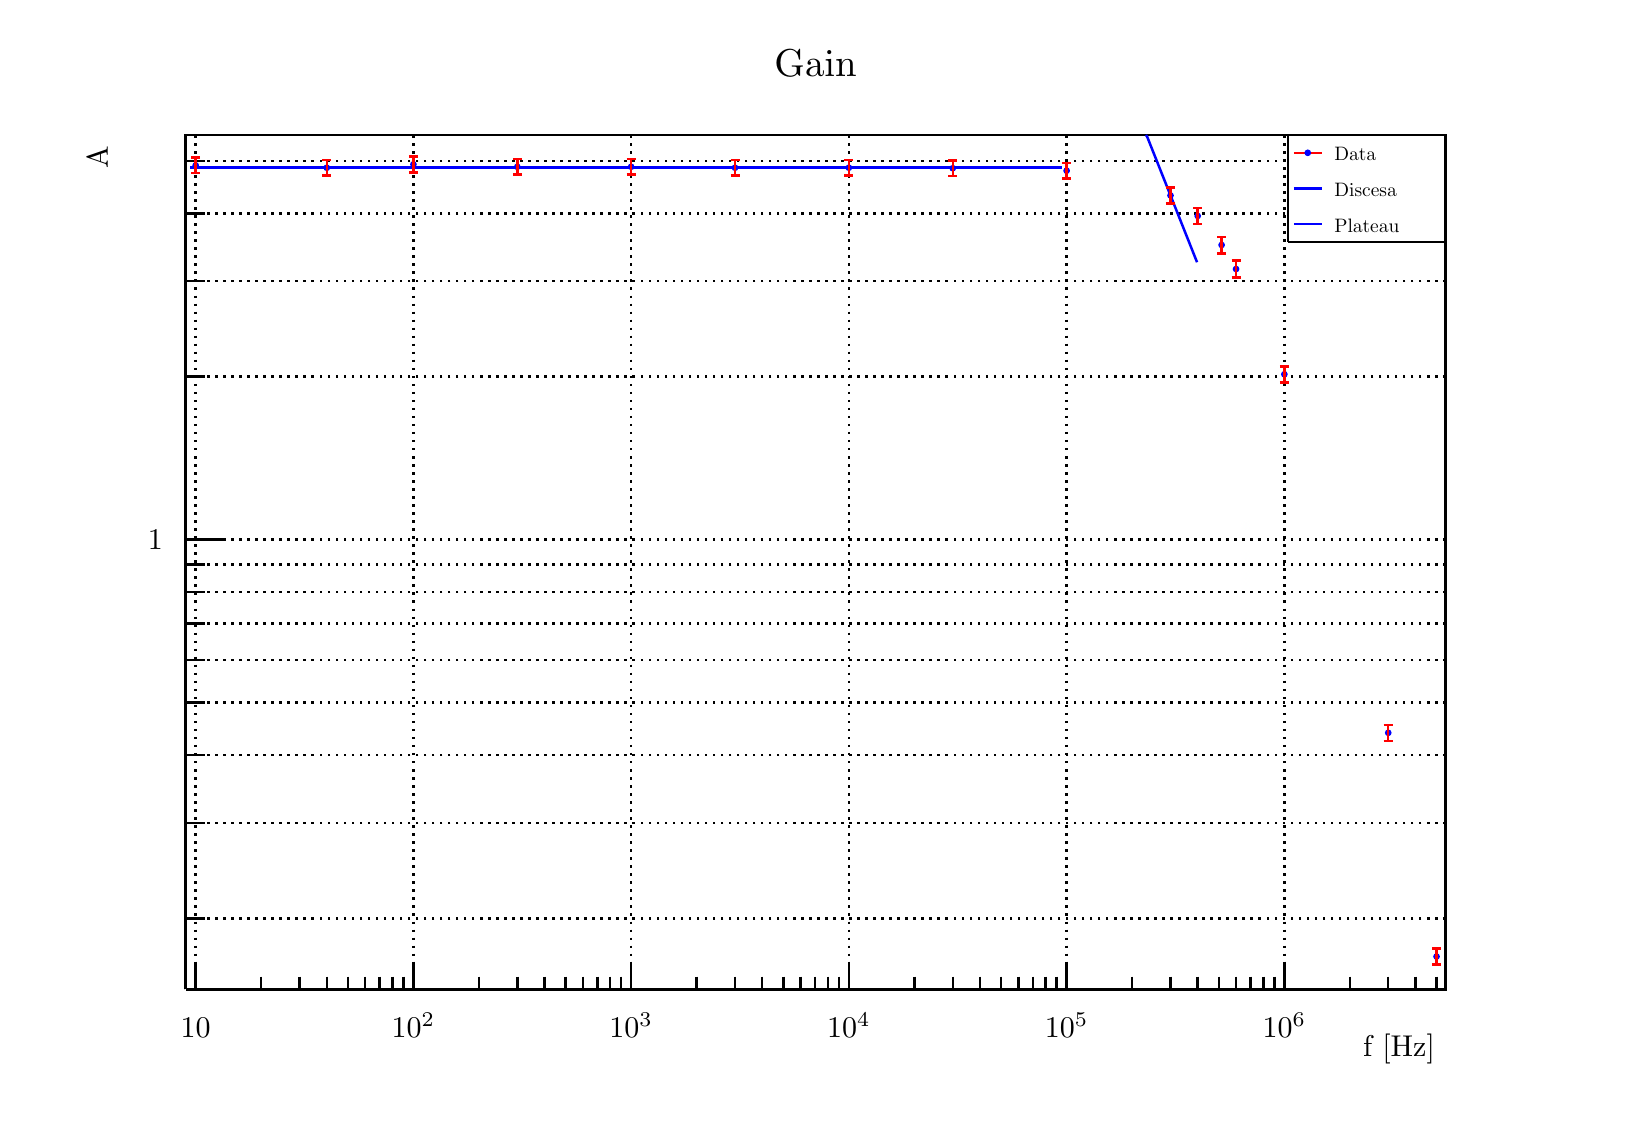
\begin{tikzpicture}
\pgfdeclareplotmark{cross} {
\pgfpathmoveto{\pgfpoint{-0.3\pgfplotmarksize}{\pgfplotmarksize}}
\pgfpathlineto{\pgfpoint{+0.3\pgfplotmarksize}{\pgfplotmarksize}}
\pgfpathlineto{\pgfpoint{+0.3\pgfplotmarksize}{0.3\pgfplotmarksize}}
\pgfpathlineto{\pgfpoint{+1\pgfplotmarksize}{0.3\pgfplotmarksize}}
\pgfpathlineto{\pgfpoint{+1\pgfplotmarksize}{-0.3\pgfplotmarksize}}
\pgfpathlineto{\pgfpoint{+0.3\pgfplotmarksize}{-0.3\pgfplotmarksize}}
\pgfpathlineto{\pgfpoint{+0.3\pgfplotmarksize}{-1.\pgfplotmarksize}}
\pgfpathlineto{\pgfpoint{-0.3\pgfplotmarksize}{-1.\pgfplotmarksize}}
\pgfpathlineto{\pgfpoint{-0.3\pgfplotmarksize}{-0.3\pgfplotmarksize}}
\pgfpathlineto{\pgfpoint{-1.\pgfplotmarksize}{-0.3\pgfplotmarksize}}
\pgfpathlineto{\pgfpoint{-1.\pgfplotmarksize}{0.3\pgfplotmarksize}}
\pgfpathlineto{\pgfpoint{-0.3\pgfplotmarksize}{0.3\pgfplotmarksize}}
\pgfpathclose
\pgfusepathqstroke
}
\pgfdeclareplotmark{cross*} {
\pgfpathmoveto{\pgfpoint{-0.3\pgfplotmarksize}{\pgfplotmarksize}}
\pgfpathlineto{\pgfpoint{+0.3\pgfplotmarksize}{\pgfplotmarksize}}
\pgfpathlineto{\pgfpoint{+0.3\pgfplotmarksize}{0.3\pgfplotmarksize}}
\pgfpathlineto{\pgfpoint{+1\pgfplotmarksize}{0.3\pgfplotmarksize}}
\pgfpathlineto{\pgfpoint{+1\pgfplotmarksize}{-0.3\pgfplotmarksize}}
\pgfpathlineto{\pgfpoint{+0.3\pgfplotmarksize}{-0.3\pgfplotmarksize}}
\pgfpathlineto{\pgfpoint{+0.3\pgfplotmarksize}{-1.\pgfplotmarksize}}
\pgfpathlineto{\pgfpoint{-0.3\pgfplotmarksize}{-1.\pgfplotmarksize}}
\pgfpathlineto{\pgfpoint{-0.3\pgfplotmarksize}{-0.3\pgfplotmarksize}}
\pgfpathlineto{\pgfpoint{-1.\pgfplotmarksize}{-0.3\pgfplotmarksize}}
\pgfpathlineto{\pgfpoint{-1.\pgfplotmarksize}{0.3\pgfplotmarksize}}
\pgfpathlineto{\pgfpoint{-0.3\pgfplotmarksize}{0.3\pgfplotmarksize}}
\pgfpathclose
\pgfusepathqfillstroke
}
\pgfdeclareplotmark{newstar} {
\pgfpathmoveto{\pgfqpoint{0pt}{\pgfplotmarksize}}
\pgfpathlineto{\pgfqpointpolar{44}{0.5\pgfplotmarksize}}
\pgfpathlineto{\pgfqpointpolar{18}{\pgfplotmarksize}}
\pgfpathlineto{\pgfqpointpolar{-20}{0.5\pgfplotmarksize}}
\pgfpathlineto{\pgfqpointpolar{-54}{\pgfplotmarksize}}
\pgfpathlineto{\pgfqpointpolar{-90}{0.5\pgfplotmarksize}}
\pgfpathlineto{\pgfqpointpolar{234}{\pgfplotmarksize}}
\pgfpathlineto{\pgfqpointpolar{198}{0.5\pgfplotmarksize}}
\pgfpathlineto{\pgfqpointpolar{162}{\pgfplotmarksize}}
\pgfpathlineto{\pgfqpointpolar{134}{0.5\pgfplotmarksize}}
\pgfpathclose
\pgfusepathqstroke
}
\pgfdeclareplotmark{newstar*} {
\pgfpathmoveto{\pgfqpoint{0pt}{\pgfplotmarksize}}
\pgfpathlineto{\pgfqpointpolar{44}{0.5\pgfplotmarksize}}
\pgfpathlineto{\pgfqpointpolar{18}{\pgfplotmarksize}}
\pgfpathlineto{\pgfqpointpolar{-20}{0.5\pgfplotmarksize}}
\pgfpathlineto{\pgfqpointpolar{-54}{\pgfplotmarksize}}
\pgfpathlineto{\pgfqpointpolar{-90}{0.5\pgfplotmarksize}}
\pgfpathlineto{\pgfqpointpolar{234}{\pgfplotmarksize}}
\pgfpathlineto{\pgfqpointpolar{198}{0.5\pgfplotmarksize}}
\pgfpathlineto{\pgfqpointpolar{162}{\pgfplotmarksize}}
\pgfpathlineto{\pgfqpointpolar{134}{0.5\pgfplotmarksize}}
\pgfpathclose
\pgfusepathqfillstroke
}
\definecolor{c}{rgb}{1,1,1};
\draw [color=c, fill=c] (0,0) rectangle (20,13.5632);
\draw [color=c, fill=c] (2,1.35632) rectangle (18,12.2069);
\definecolor{c}{rgb}{0,0,0};
\draw [c,line width=0.9] (2,1.35632) -- (2,12.2069) -- (18,12.2069) -- (18,1.35632) -- (2,1.35632);
\definecolor{c}{rgb}{1,1,1};
\draw [color=c, fill=c] (2,1.35632) rectangle (18,12.2069);
\definecolor{c}{rgb}{0,0,0};
\draw [c,line width=0.9] (2,1.35632) -- (2,12.2069) -- (18,12.2069) -- (18,1.35632) -- (2,1.35632);
\draw [c,line width=0.9] (2,1.35632) -- (18,1.35632);
\draw [c,dotted,line width=0.9] (2.12653,12.2069) -- (2.12653,1.35632);
\draw [c,dotted,line width=0.9] (4.89177,12.2069) -- (4.89177,1.35632);
\draw [c,dotted,line width=0.9] (7.657,12.2069) -- (7.657,1.35632);
\draw [c,dotted,line width=0.9] (10.4222,12.2069) -- (10.4222,1.35632);
\draw [c,dotted,line width=0.9] (13.1875,12.2069) -- (13.1875,1.35632);
\draw [c,dotted,line width=0.9] (15.9527,12.2069) -- (15.9527,1.35632);
\draw [c,line width=0.9] (2,1.35632) -- (2,12.2069);
\draw [c,dotted,line width=0.9] (18,2.25939) -- (2,2.25939);
\draw [c,dotted,line width=0.9] (18,3.47074) -- (2,3.47074);
\draw [c,dotted,line width=0.9] (18,4.3302) -- (2,4.3302);
\draw [c,dotted,line width=0.9] (18,4.99685) -- (2,4.99685);
\draw [c,dotted,line width=0.9] (18,5.54154) -- (2,5.54154);
\draw [c,dotted,line width=0.9] (18,6.00207) -- (2,6.00207);
\draw [c,dotted,line width=0.9] (18,6.401) -- (2,6.401);
\draw [c,dotted,line width=0.9] (18,6.75288) -- (2,6.75288);
\draw [c,dotted,line width=0.9] (18,7.06765) -- (2,7.06765);
\draw [c,dotted,line width=0.9] (18,9.13846) -- (2,9.13846);
\draw [c,dotted,line width=0.9] (18,10.3498) -- (2,10.3498);
\draw [c,dotted,line width=0.9] (18,11.2093) -- (2,11.2093);
\draw [c,dotted,line width=0.9] (18,11.8759) -- (2,11.8759);
\draw [c,line width=0.9] (2,1.35632) -- (18,1.35632);
\draw [anchor= east] (18,0.596782) node[scale=1.08496, color=c, rotate=0]{f [Hz]};
\draw [c,line width=0.9] (2.12653,1.68184) -- (2.12653,1.35632);
\draw [anchor=base] (2.12653,0.742586) node[scale=1.08496, color=c, rotate=0]{10};
\draw [c,line width=0.9] (2.95895,1.51908) -- (2.95895,1.35632);
\draw [c,line width=0.9] (3.44588,1.51908) -- (3.44588,1.35632);
\draw [c,line width=0.9] (3.79137,1.51908) -- (3.79137,1.35632);
\draw [c,line width=0.9] (4.05935,1.51908) -- (4.05935,1.35632);
\draw [c,line width=0.9] (4.2783,1.51908) -- (4.2783,1.35632);
\draw [c,line width=0.9] (4.46343,1.51908) -- (4.46343,1.35632);
\draw [c,line width=0.9] (4.62379,1.51908) -- (4.62379,1.35632);
\draw [c,line width=0.9] (4.76524,1.51908) -- (4.76524,1.35632);
\draw [c,line width=0.9] (4.89177,1.68184) -- (4.89177,1.35632);
\draw [anchor=base] (4.89177,0.742586) node[scale=1.08496, color=c, rotate=0]{$10^{2}$};
\draw [c,line width=0.9] (5.72419,1.51908) -- (5.72419,1.35632);
\draw [c,line width=0.9] (6.21112,1.51908) -- (6.21112,1.35632);
\draw [c,line width=0.9] (6.55661,1.51908) -- (6.55661,1.35632);
\draw [c,line width=0.9] (6.82458,1.51908) -- (6.82458,1.35632);
\draw [c,line width=0.9] (7.04354,1.51908) -- (7.04354,1.35632);
\draw [c,line width=0.9] (7.22866,1.51908) -- (7.22866,1.35632);
\draw [c,line width=0.9] (7.38903,1.51908) -- (7.38903,1.35632);
\draw [c,line width=0.9] (7.53047,1.51908) -- (7.53047,1.35632);
\draw [c,line width=0.9] (7.657,1.68184) -- (7.657,1.35632);
\draw [anchor=base] (7.657,0.742586) node[scale=1.08496, color=c, rotate=0]{$10^{3}$};
\draw [c,line width=0.9] (8.48942,1.51908) -- (8.48942,1.35632);
\draw [c,line width=0.9] (8.97636,1.51908) -- (8.97636,1.35632);
\draw [c,line width=0.9] (9.32184,1.51908) -- (9.32184,1.35632);
\draw [c,line width=0.9] (9.58982,1.51908) -- (9.58982,1.35632);
\draw [c,line width=0.9] (9.80878,1.51908) -- (9.80878,1.35632);
\draw [c,line width=0.9] (9.9939,1.51908) -- (9.9939,1.35632);
\draw [c,line width=0.9] (10.1543,1.51908) -- (10.1543,1.35632);
\draw [c,line width=0.9] (10.2957,1.51908) -- (10.2957,1.35632);
\draw [c,line width=0.9] (10.4222,1.68184) -- (10.4222,1.35632);
\draw [anchor=base] (10.4222,0.742586) node[scale=1.08496, color=c, rotate=0]{$10^{4}$};
\draw [c,line width=0.9] (11.2547,1.51908) -- (11.2547,1.35632);
\draw [c,line width=0.9] (11.7416,1.51908) -- (11.7416,1.35632);
\draw [c,line width=0.9] (12.0871,1.51908) -- (12.0871,1.35632);
\draw [c,line width=0.9] (12.3551,1.51908) -- (12.3551,1.35632);
\draw [c,line width=0.9] (12.574,1.51908) -- (12.574,1.35632);
\draw [c,line width=0.9] (12.7591,1.51908) -- (12.7591,1.35632);
\draw [c,line width=0.9] (12.9195,1.51908) -- (12.9195,1.35632);
\draw [c,line width=0.9] (13.061,1.51908) -- (13.061,1.35632);
\draw [c,line width=0.9] (13.1875,1.68184) -- (13.1875,1.35632);
\draw [anchor=base] (13.1875,0.742586) node[scale=1.08496, color=c, rotate=0]{$10^{5}$};
\draw [c,line width=0.9] (14.0199,1.51908) -- (14.0199,1.35632);
\draw [c,line width=0.9] (14.5068,1.51908) -- (14.5068,1.35632);
\draw [c,line width=0.9] (14.8523,1.51908) -- (14.8523,1.35632);
\draw [c,line width=0.9] (15.1203,1.51908) -- (15.1203,1.35632);
\draw [c,line width=0.9] (15.3393,1.51908) -- (15.3393,1.35632);
\draw [c,line width=0.9] (15.5244,1.51908) -- (15.5244,1.35632);
\draw [c,line width=0.9] (15.6847,1.51908) -- (15.6847,1.35632);
\draw [c,line width=0.9] (15.8262,1.51908) -- (15.8262,1.35632);
\draw [c,line width=0.9] (15.9527,1.68184) -- (15.9527,1.35632);
\draw [anchor=base] (15.9527,0.742586) node[scale=1.08496, color=c, rotate=0]{$10^{6}$};
\draw [c,line width=0.9] (16.7851,1.51908) -- (16.7851,1.35632);
\draw [c,line width=0.9] (17.2721,1.51908) -- (17.2721,1.35632);
\draw [c,line width=0.9] (17.6176,1.51908) -- (17.6176,1.35632);
\draw [c,line width=0.9] (17.8855,1.51908) -- (17.8855,1.35632);
\draw [c,line width=0.9] (2,1.35632) -- (2,12.2069);
\draw [anchor= east] (0.88,12.2069) node[scale=1.08496, color=c, rotate=90]{A};
\draw [c,line width=0.9] (2.24,2.25939) -- (2,2.25939);
\draw [c,line width=0.9] (2.24,3.47074) -- (2,3.47074);
\draw [c,line width=0.9] (2.24,4.3302) -- (2,4.3302);
\draw [c,line width=0.9] (2.24,4.99685) -- (2,4.99685);
\draw [c,line width=0.9] (2.24,5.54154) -- (2,5.54154);
\draw [c,line width=0.9] (2.24,6.00207) -- (2,6.00207);
\draw [c,line width=0.9] (2.24,6.401) -- (2,6.401);
\draw [c,line width=0.9] (2.24,6.75288) -- (2,6.75288);
\draw [c,line width=0.9] (2.48,7.06765) -- (2,7.06765);
\draw [anchor= east] (1.844,7.06765) node[scale=1.08496, color=c, rotate=0]{1};
\draw [c,line width=0.9] (2.24,9.13846) -- (2,9.13846);
\draw [c,line width=0.9] (2.24,10.3498) -- (2,10.3498);
\draw [c,line width=0.9] (2.24,11.2093) -- (2,11.2093);
\draw [c,line width=0.9] (2.24,11.8759) -- (2,11.8759);
\definecolor{c}{rgb}{0,0,1};
\foreach \P in {(2.12653,11.8216), (3.79137,11.7911), (4.89177,11.8338), (6.21112,11.8033), (7.65701,11.8033), (8.97636,11.7911), (10.4222,11.7911), (11.7416,11.7849), (13.1875,11.754), (14.5068,11.4392), (14.8523,11.1792), (15.1558,10.8103),
 (15.3393,10.505), (15.9527,9.16818), (17.2721,4.61494), (17.8855,1.77386)}{\draw[mark options={color=c,fill=c},mark size=1.681682pt,mark=*,mark size=1pt] plot coordinates {\P};}
\draw [c,line width=0.9] (2.05724,11.7969) -- (2.16911,11.7969) -- (2.28099,11.7969) -- (2.39286,11.7969) -- (2.50474,11.7969) -- (2.61661,11.7969) -- (2.72849,11.7969) -- (2.84036,11.7969) -- (2.95224,11.7969) -- (3.06411,11.7969) --
 (3.17599,11.7969) -- (3.28786,11.7969) -- (3.39974,11.7969) -- (3.51161,11.7969) -- (3.62349,11.7969) -- (3.73536,11.7969) -- (3.84724,11.7969) -- (3.95911,11.7969) -- (4.07099,11.7969) -- (4.18286,11.7969) -- (4.29474,11.7969) -- (4.40661,11.7969)
 -- (4.51849,11.7969) -- (4.63036,11.7969) -- (4.74224,11.7969) -- (4.85411,11.7969) -- (4.96599,11.7969) -- (5.07786,11.7969) -- (5.18974,11.7969) -- (5.30161,11.7969) -- (5.41349,11.7969) -- (5.52536,11.7969) -- (5.63724,11.7969) --
 (5.74911,11.7969) -- (5.86099,11.7969) -- (5.97286,11.7969) -- (6.08474,11.7969) -- (6.19661,11.7969) -- (6.30849,11.7969) -- (6.42036,11.7969) -- (6.53224,11.7969) -- (6.64411,11.7969) -- (6.75599,11.7969) -- (6.86786,11.7969) -- (6.97974,11.7969)
 -- (7.09161,11.7969) -- (7.20349,11.7969) -- (7.31536,11.7969) -- (7.42724,11.7969) -- (7.53911,11.7969);
\draw [c,line width=0.9] (7.53911,11.7969) -- (7.65099,11.7969) -- (7.76286,11.7969) -- (7.87474,11.7969) -- (7.98661,11.7969) -- (8.09849,11.7969) -- (8.21036,11.7969) -- (8.32224,11.7969) -- (8.43411,11.7969) -- (8.54599,11.7969) --
 (8.65786,11.7969) -- (8.76974,11.7969) -- (8.88161,11.7969) -- (8.99349,11.7969) -- (9.10536,11.7969) -- (9.21724,11.7969) -- (9.32911,11.7969) -- (9.44099,11.7969) -- (9.55286,11.7969) -- (9.66474,11.7969) -- (9.77661,11.7969) -- (9.88849,11.7969)
 -- (10.0004,11.7969) -- (10.1122,11.7969) -- (10.2241,11.7969) -- (10.336,11.7969) -- (10.4479,11.7969) -- (10.5597,11.7969) -- (10.6716,11.7969) -- (10.7835,11.7969) -- (10.8954,11.7969) -- (11.0072,11.7969) -- (11.1191,11.7969) -- (11.231,11.7969)
 -- (11.3429,11.7969) -- (11.4547,11.7969) -- (11.5666,11.7969) -- (11.6785,11.7969) -- (11.7904,11.7969) -- (11.9022,11.7969) -- (12.0141,11.7969) -- (12.126,11.7969) -- (12.2379,11.7969) -- (12.3497,11.7969) -- (12.4616,11.7969) --
 (12.5735,11.7969) -- (12.6854,11.7969) -- (12.7972,11.7969) -- (12.9091,11.7969) -- (13.021,11.7969);
\draw [c,line width=0.9] (13.021,11.7969) -- (13.1329,11.7969);
\draw [c,line width=0.9] (14.1947,12.2069) -- (14.2114,12.1824) -- (14.228,12.1405) -- (14.2447,12.0986) -- (14.2613,12.0567) -- (14.278,12.0149) -- (14.2946,11.973) -- (14.3113,11.9311) -- (14.3279,11.8892) -- (14.3446,11.8474) -- (14.3612,11.8055)
 -- (14.3779,11.7636) -- (14.3945,11.7217) -- (14.4112,11.6798) -- (14.4278,11.638) -- (14.4445,11.5961) -- (14.4611,11.5542) -- (14.4778,11.5123) -- (14.4944,11.4704) -- (14.5111,11.4286) -- (14.5277,11.3867) -- (14.5444,11.3448) -- (14.561,11.3029)
 -- (14.5777,11.2611) -- (14.5943,11.2192) -- (14.6109,11.1773) -- (14.6276,11.1354) -- (14.6442,11.0935) -- (14.6609,11.0517) -- (14.6775,11.0098) -- (14.6942,10.9679) -- (14.7108,10.926) -- (14.7275,10.8841) -- (14.7441,10.8423) --
 (14.7608,10.8004) -- (14.7774,10.7585) -- (14.7941,10.7166) -- (14.8107,10.6748) -- (14.8274,10.6329) -- (14.844,10.591);
\definecolor{c}{rgb}{1,0,0};
\draw [c,line width=0.9] (2.12653,11.8216) -- (2.12653,11.9188);
\draw [c,line width=0.9] (2.06906,11.9188) -- (2.184,11.9188);
\draw [c,line width=0.9] (2.12653,11.8216) -- (2.12653,11.7212);
\draw [c,line width=0.9] (2.06906,11.7212) -- (2.184,11.7212);
\draw [c,line width=0.9] (3.79137,11.7911) -- (3.79137,11.8884);
\draw [c,line width=0.9] (3.7339,11.8884) -- (3.84884,11.8884);
\draw [c,line width=0.9] (3.79137,11.7911) -- (3.79137,11.6905);
\draw [c,line width=0.9] (3.7339,11.6905) -- (3.84884,11.6905);
\draw [c,line width=0.9] (4.89177,11.8338) -- (4.89177,11.9309);
\draw [c,line width=0.9] (4.8343,11.9309) -- (4.94924,11.9309);
\draw [c,line width=0.9] (4.89177,11.8338) -- (4.89177,11.7334);
\draw [c,line width=0.9] (4.8343,11.7334) -- (4.94924,11.7334);
\draw [c,line width=0.9] (6.21112,11.8033) -- (6.21112,11.9006);
\draw [c,line width=0.9] (6.15365,11.9006) -- (6.26859,11.9006);
\draw [c,line width=0.9] (6.21112,11.8033) -- (6.21112,11.7028);
\draw [c,line width=0.9] (6.15365,11.7028) -- (6.26859,11.7028);
\draw [c,line width=0.9] (7.65701,11.8033) -- (7.65701,11.9006);
\draw [c,line width=0.9] (7.59954,11.9006) -- (7.71448,11.9006);
\draw [c,line width=0.9] (7.65701,11.8033) -- (7.65701,11.7028);
\draw [c,line width=0.9] (7.59954,11.7028) -- (7.71448,11.7028);
\draw [c,line width=0.9] (8.97636,11.7911) -- (8.97636,11.8884);
\draw [c,line width=0.9] (8.91889,11.8884) -- (9.03383,11.8884);
\draw [c,line width=0.9] (8.97636,11.7911) -- (8.97636,11.6905);
\draw [c,line width=0.9] (8.91889,11.6905) -- (9.03383,11.6905);
\draw [c,line width=0.9] (10.4222,11.7911) -- (10.4222,11.8884);
\draw [c,line width=0.9] (10.3648,11.8884) -- (10.4797,11.8884);
\draw [c,line width=0.9] (10.4222,11.7911) -- (10.4222,11.6905);
\draw [c,line width=0.9] (10.3648,11.6905) -- (10.4797,11.6905);
\draw [c,line width=0.9] (11.7416,11.7849) -- (11.7416,11.8823);
\draw [c,line width=0.9] (11.6841,11.8823) -- (11.7991,11.8823);
\draw [c,line width=0.9] (11.7416,11.7849) -- (11.7416,11.6843);
\draw [c,line width=0.9] (11.6841,11.6843) -- (11.7991,11.6843);
\draw [c,line width=0.9] (13.1875,11.754) -- (13.1875,11.8514);
\draw [c,line width=0.9] (13.13,11.8514) -- (13.245,11.8514);
\draw [c,line width=0.9] (13.1875,11.754) -- (13.1875,11.6532);
\draw [c,line width=0.9] (13.13,11.6532) -- (13.245,11.6532);
\draw [c,line width=0.9] (14.5068,11.4392) -- (14.5068,11.5383);
\draw [c,line width=0.9] (14.4494,11.5383) -- (14.5643,11.5383);
\draw [c,line width=0.9] (14.5068,11.4392) -- (14.5068,11.3367);
\draw [c,line width=0.9] (14.4494,11.3367) -- (14.5643,11.3367);
\draw [c,line width=0.9] (14.8523,11.1792) -- (14.8523,11.2799);
\draw [c,line width=0.9] (14.7949,11.2799) -- (14.9098,11.2799);
\draw [c,line width=0.9] (14.8523,11.1792) -- (14.8523,11.0751);
\draw [c,line width=0.9] (14.7949,11.0751) -- (14.9098,11.0751);
\draw [c,line width=0.9] (15.1558,10.8103) -- (15.1558,10.9136);
\draw [c,line width=0.9] (15.0983,10.9136) -- (15.2133,10.9136);
\draw [c,line width=0.9] (15.1558,10.8103) -- (15.1558,10.7033);
\draw [c,line width=0.9] (15.0983,10.7033) -- (15.2133,10.7033);
\draw [c,line width=0.9] (15.3393,10.505) -- (15.3393,10.611);
\draw [c,line width=0.9] (15.2818,10.611) -- (15.3967,10.611);
\draw [c,line width=0.9] (15.3393,10.505) -- (15.3393,10.3951);
\draw [c,line width=0.9] (15.2818,10.3951) -- (15.3967,10.3951);
\draw [c,line width=0.9] (15.9527,9.16818) -- (15.9527,9.26843);
\draw [c,line width=0.9] (15.8952,9.26843) -- (16.0102,9.26843);
\draw [c,line width=0.9] (15.9527,9.16818) -- (15.9527,9.06445);
\draw [c,line width=0.9] (15.8952,9.06445) -- (16.0102,9.06445);
\draw [c,line width=0.9] (17.2721,4.61494) -- (17.2721,4.71371);
\draw [c,line width=0.9] (17.2146,4.71371) -- (17.3295,4.71371);
\draw [c,line width=0.9] (17.2721,4.61494) -- (17.2721,4.51278);
\draw [c,line width=0.9] (17.2146,4.51278) -- (17.3295,4.51278);
\draw [c,line width=0.9] (17.8855,1.77386) -- (17.8855,1.8732);
\draw [c,line width=0.9] (17.8281,1.8732) -- (17.943,1.8732);
\draw [c,line width=0.9] (17.8855,1.77386) -- (17.8855,1.67109);
\draw [c,line width=0.9] (17.8281,1.67109) -- (17.943,1.67109);
\definecolor{c}{rgb}{1,1,1};
\draw [color=c, fill=c] (16,10.8506) rectangle (18,12.2069);
\definecolor{c}{rgb}{0,0,0};
\draw [c,line width=0.9] (16,10.8506) -- (18,10.8506);
\draw [c,line width=0.9] (18,10.8506) -- (18,12.2069);
\draw [c,line width=0.9] (18,12.2069) -- (16,12.2069);
\draw [c,line width=0.9] (16,12.2069) -- (16,10.8506);
\draw [anchor=base west] (16.5,11.8791) node[scale=0.702031, color=c, rotate=0]{Data};
\definecolor{c}{rgb}{1,0,0};
\draw [c,line width=0.9] (16.075,11.9808) -- (16.425,11.9808);
\definecolor{c}{rgb}{0,0,1};
\foreach \P in {(16.25,11.9808)}{\draw[mark options={color=c,fill=c},mark size=1.681682pt,mark=*,mark size=1pt] plot coordinates {\P};}
\definecolor{c}{rgb}{0,0,0};
\draw [anchor=base west] (16.5,11.427) node[scale=0.702031, color=c, rotate=0]{Discesa};
\definecolor{c}{rgb}{0,0,1};
\draw [c,line width=0.9] (16.075,11.5287) -- (16.425,11.5287);
\definecolor{c}{rgb}{0,0,0};
\draw [anchor=base west] (16.5,10.9749) node[scale=0.702031, color=c, rotate=0]{Plateau};
\definecolor{c}{rgb}{0,0,1};
\draw [c,line width=0.9] (16.075,11.0766) -- (16.425,11.0766);
\definecolor{c}{rgb}{0,0,0};
\draw (10,13.1224) node[scale=1.40406, color=c, rotate=0]{Gain};
\end{tikzpicture}
 
 \caption{Risposta in frequenza di un amplificatore non invertente con A=5} 
 \label{gr:amp_noninv_A5.tex} 
\end{grafico}

\begin{tabella}
 \centering
  \begin{center}
\begin{tabulary}{\textwidth}{CC}
\toprule
f(Hz) & A  \\ \midrule
10 & 4.91  \\ \midrule
40 & 4.86  \\ \midrule
100 & 4.93  \\ \midrule
300 & 4.88  \\ \midrule
1000 & 4.88  \\ \midrule
3000 & 4.86  \\ \midrule
10000 & 4.86 \\ \midrule
30000 & 4.85  \\ \midrule
100000 & 4.8  \\ \midrule
300000 & 4.32  \\ \midrule
400000 & 3.96  \\ \midrule
515000 & 3.50  \\ \midrule
600000 & 3.16  \\ \midrule
1000000 & 2.02  \\ \midrule
3000000 & 0.44  \\ \midrule
5000000 & 0.17  \\ \midrule
 \bottomrule
\end{tabulary}
\end{center}



 
 \caption{Dati risposta in frequenza}
 \label{tab:tab_noninv_A5.tex}
\end{tabella}

Sono state interpolate separatamente la zona di plateau e di discesa, ottenendo come risultati:
$A_{plateau}=quel che è \pm$
%inserire retta interpolante

Dall'interpolazione si è poi ricavato 
$f_b= \pm \,Hz $
Il GBP è
$GBP=A_{CL} \cdot f_b $


\subsection{Amplificatore con A=1}
Le resistenze inserite sono state sostituite con:
$R_{1,up}=32.6 \pm 0.2 \,k\Omega $%mettere errore
$R_{1,down}=32.6 \pm 0.2\,k\Omega$ %mettere errore
$R_{2,up}=32.7 \pm 0.2\,k\Omega$ %mettere errore
$R_{2,down}=32.5 \pm 0.2\,k\Omega$
$R_4=56.0 \pm 0.3\,\Omega$
\begin{grafico}
 \centering 
 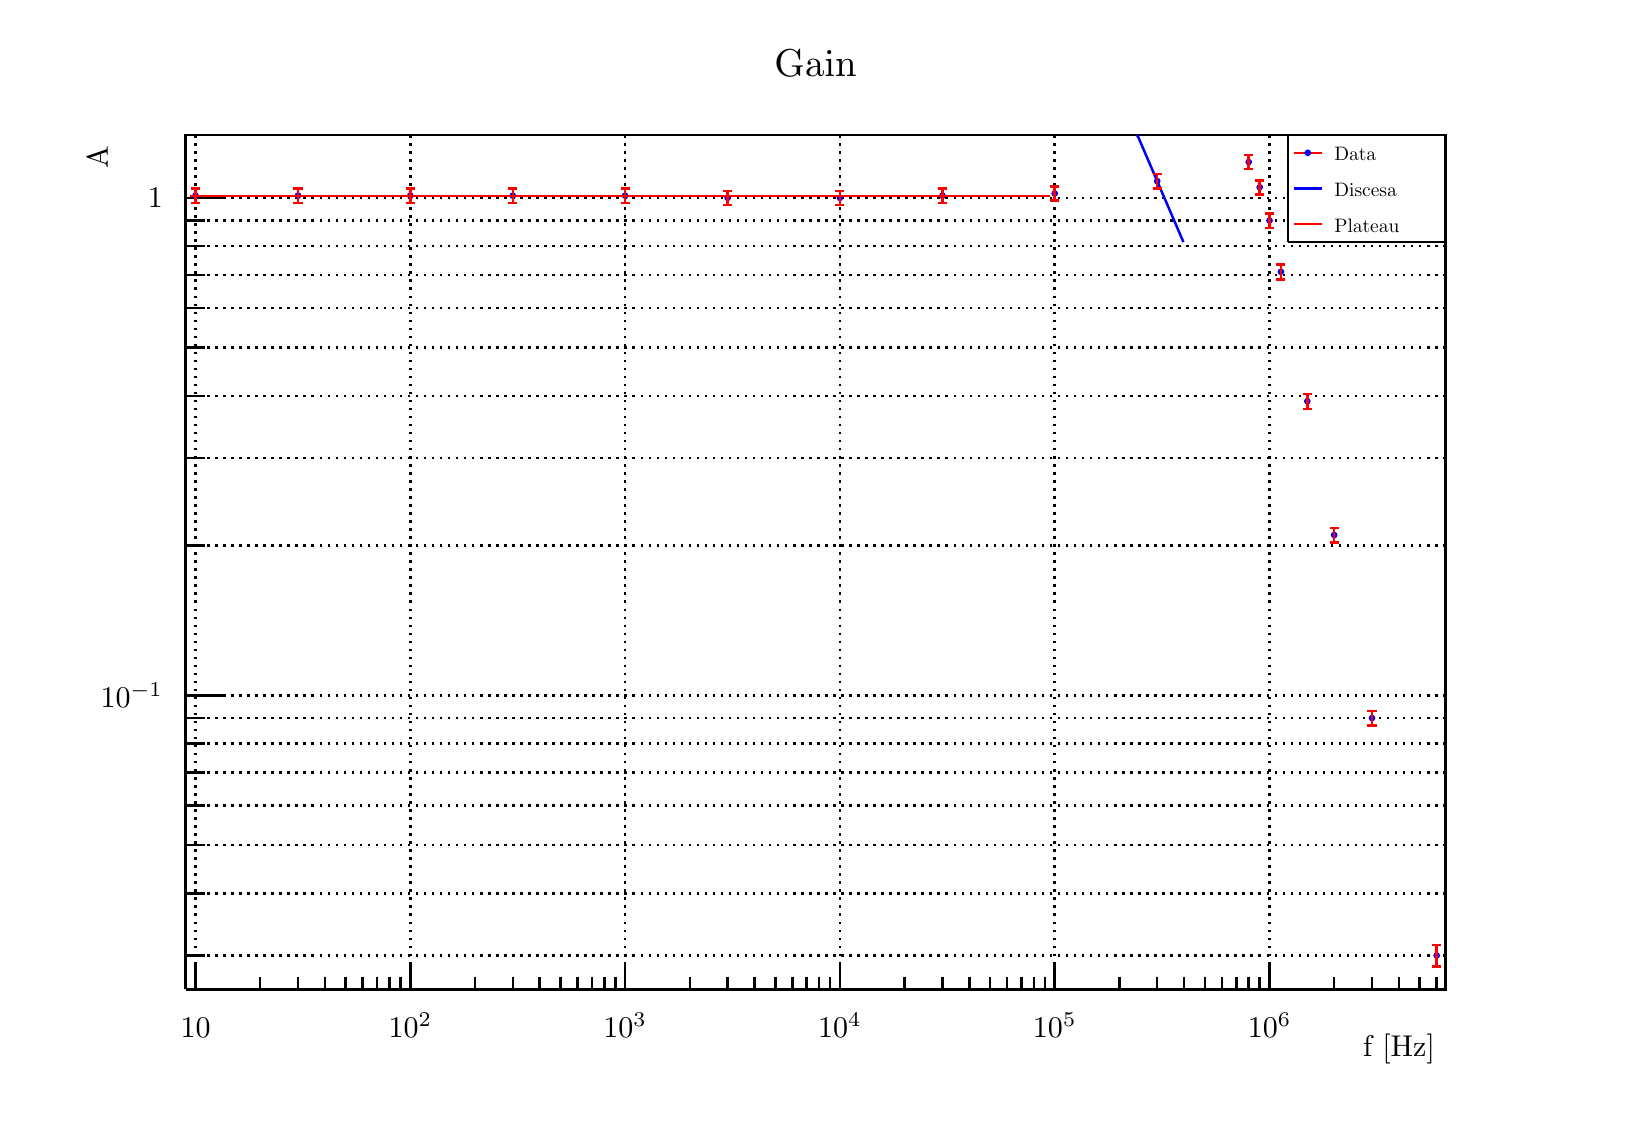
\begin{tikzpicture}
\pgfdeclareplotmark{cross} {
\pgfpathmoveto{\pgfpoint{-0.3\pgfplotmarksize}{\pgfplotmarksize}}
\pgfpathlineto{\pgfpoint{+0.3\pgfplotmarksize}{\pgfplotmarksize}}
\pgfpathlineto{\pgfpoint{+0.3\pgfplotmarksize}{0.3\pgfplotmarksize}}
\pgfpathlineto{\pgfpoint{+1\pgfplotmarksize}{0.3\pgfplotmarksize}}
\pgfpathlineto{\pgfpoint{+1\pgfplotmarksize}{-0.3\pgfplotmarksize}}
\pgfpathlineto{\pgfpoint{+0.3\pgfplotmarksize}{-0.3\pgfplotmarksize}}
\pgfpathlineto{\pgfpoint{+0.3\pgfplotmarksize}{-1.\pgfplotmarksize}}
\pgfpathlineto{\pgfpoint{-0.3\pgfplotmarksize}{-1.\pgfplotmarksize}}
\pgfpathlineto{\pgfpoint{-0.3\pgfplotmarksize}{-0.3\pgfplotmarksize}}
\pgfpathlineto{\pgfpoint{-1.\pgfplotmarksize}{-0.3\pgfplotmarksize}}
\pgfpathlineto{\pgfpoint{-1.\pgfplotmarksize}{0.3\pgfplotmarksize}}
\pgfpathlineto{\pgfpoint{-0.3\pgfplotmarksize}{0.3\pgfplotmarksize}}
\pgfpathclose
\pgfusepathqstroke
}
\pgfdeclareplotmark{cross*} {
\pgfpathmoveto{\pgfpoint{-0.3\pgfplotmarksize}{\pgfplotmarksize}}
\pgfpathlineto{\pgfpoint{+0.3\pgfplotmarksize}{\pgfplotmarksize}}
\pgfpathlineto{\pgfpoint{+0.3\pgfplotmarksize}{0.3\pgfplotmarksize}}
\pgfpathlineto{\pgfpoint{+1\pgfplotmarksize}{0.3\pgfplotmarksize}}
\pgfpathlineto{\pgfpoint{+1\pgfplotmarksize}{-0.3\pgfplotmarksize}}
\pgfpathlineto{\pgfpoint{+0.3\pgfplotmarksize}{-0.3\pgfplotmarksize}}
\pgfpathlineto{\pgfpoint{+0.3\pgfplotmarksize}{-1.\pgfplotmarksize}}
\pgfpathlineto{\pgfpoint{-0.3\pgfplotmarksize}{-1.\pgfplotmarksize}}
\pgfpathlineto{\pgfpoint{-0.3\pgfplotmarksize}{-0.3\pgfplotmarksize}}
\pgfpathlineto{\pgfpoint{-1.\pgfplotmarksize}{-0.3\pgfplotmarksize}}
\pgfpathlineto{\pgfpoint{-1.\pgfplotmarksize}{0.3\pgfplotmarksize}}
\pgfpathlineto{\pgfpoint{-0.3\pgfplotmarksize}{0.3\pgfplotmarksize}}
\pgfpathclose
\pgfusepathqfillstroke
}
\pgfdeclareplotmark{newstar} {
\pgfpathmoveto{\pgfqpoint{0pt}{\pgfplotmarksize}}
\pgfpathlineto{\pgfqpointpolar{44}{0.5\pgfplotmarksize}}
\pgfpathlineto{\pgfqpointpolar{18}{\pgfplotmarksize}}
\pgfpathlineto{\pgfqpointpolar{-20}{0.5\pgfplotmarksize}}
\pgfpathlineto{\pgfqpointpolar{-54}{\pgfplotmarksize}}
\pgfpathlineto{\pgfqpointpolar{-90}{0.5\pgfplotmarksize}}
\pgfpathlineto{\pgfqpointpolar{234}{\pgfplotmarksize}}
\pgfpathlineto{\pgfqpointpolar{198}{0.5\pgfplotmarksize}}
\pgfpathlineto{\pgfqpointpolar{162}{\pgfplotmarksize}}
\pgfpathlineto{\pgfqpointpolar{134}{0.5\pgfplotmarksize}}
\pgfpathclose
\pgfusepathqstroke
}
\pgfdeclareplotmark{newstar*} {
\pgfpathmoveto{\pgfqpoint{0pt}{\pgfplotmarksize}}
\pgfpathlineto{\pgfqpointpolar{44}{0.5\pgfplotmarksize}}
\pgfpathlineto{\pgfqpointpolar{18}{\pgfplotmarksize}}
\pgfpathlineto{\pgfqpointpolar{-20}{0.5\pgfplotmarksize}}
\pgfpathlineto{\pgfqpointpolar{-54}{\pgfplotmarksize}}
\pgfpathlineto{\pgfqpointpolar{-90}{0.5\pgfplotmarksize}}
\pgfpathlineto{\pgfqpointpolar{234}{\pgfplotmarksize}}
\pgfpathlineto{\pgfqpointpolar{198}{0.5\pgfplotmarksize}}
\pgfpathlineto{\pgfqpointpolar{162}{\pgfplotmarksize}}
\pgfpathlineto{\pgfqpointpolar{134}{0.5\pgfplotmarksize}}
\pgfpathclose
\pgfusepathqfillstroke
}
\definecolor{c}{rgb}{1,1,1};
\draw [color=c, fill=c] (0,0) rectangle (20,13.5632);
\draw [color=c, fill=c] (2,1.35632) rectangle (18,12.2069);
\definecolor{c}{rgb}{0,0,0};
\draw [c,line width=0.9] (2,1.35632) -- (2,12.2069) -- (18,12.2069) -- (18,1.35632) -- (2,1.35632);
\definecolor{c}{rgb}{1,1,1};
\draw [color=c, fill=c] (2,1.35632) rectangle (18,12.2069);
\definecolor{c}{rgb}{0,0,0};
\draw [c,line width=0.9] (2,1.35632) -- (2,12.2069) -- (18,12.2069) -- (18,1.35632) -- (2,1.35632);
\draw [c,line width=0.9] (2,1.35632) -- (18,1.35632);
\draw [c,dotted,line width=0.9] (2.12482,12.2069) -- (2.12482,1.35632);
\draw [c,dotted,line width=0.9] (4.85273,12.2069) -- (4.85273,1.35632);
\draw [c,dotted,line width=0.9] (7.58064,12.2069) -- (7.58064,1.35632);
\draw [c,dotted,line width=0.9] (10.3085,12.2069) -- (10.3085,1.35632);
\draw [c,dotted,line width=0.9] (13.0365,12.2069) -- (13.0365,1.35632);
\draw [c,dotted,line width=0.9] (15.7644,12.2069) -- (15.7644,1.35632);
\draw [c,line width=0.9] (2,1.35632) -- (2,12.2069);
\draw [c,dotted,line width=0.9] (18,1.78746) -- (2,1.78746);
\draw [c,dotted,line width=0.9] (18,2.57687) -- (2,2.57687);
\draw [c,dotted,line width=0.9] (18,3.18919) -- (2,3.18919);
\draw [c,dotted,line width=0.9] (18,3.68949) -- (2,3.68949);
\draw [c,dotted,line width=0.9] (18,4.11248) -- (2,4.11248);
\draw [c,dotted,line width=0.9] (18,4.4789) -- (2,4.4789);
\draw [c,dotted,line width=0.9] (18,4.8021) -- (2,4.8021);
\draw [c,dotted,line width=0.9] (18,5.09122) -- (2,5.09122);
\draw [c,dotted,line width=0.9] (18,6.99325) -- (2,6.99325);
\draw [c,dotted,line width=0.9] (18,8.10586) -- (2,8.10586);
\draw [c,dotted,line width=0.9] (18,8.89528) -- (2,8.89528);
\draw [c,dotted,line width=0.9] (18,9.50759) -- (2,9.50759);
\draw [c,dotted,line width=0.9] (18,10.0079) -- (2,10.0079);
\draw [c,dotted,line width=0.9] (18,10.4309) -- (2,10.4309);
\draw [c,dotted,line width=0.9] (18,10.7973) -- (2,10.7973);
\draw [c,dotted,line width=0.9] (18,11.1205) -- (2,11.1205);
\draw [c,dotted,line width=0.9] (18,11.4096) -- (2,11.4096);
\draw [c,line width=0.9] (2,1.35632) -- (18,1.35632);
\draw [anchor= east] (18,0.596782) node[scale=1.08496, color=c, rotate=0]{f [Hz]};
\draw [c,line width=0.9] (2.12482,1.68184) -- (2.12482,1.35632);
\draw [anchor=base] (2.12482,0.742586) node[scale=1.08496, color=c, rotate=0]{10};
\draw [c,line width=0.9] (2.946,1.51908) -- (2.946,1.35632);
\draw [c,line width=0.9] (3.42636,1.51908) -- (3.42636,1.35632);
\draw [c,line width=0.9] (3.76718,1.51908) -- (3.76718,1.35632);
\draw [c,line width=0.9] (4.03155,1.51908) -- (4.03155,1.35632);
\draw [c,line width=0.9] (4.24754,1.51908) -- (4.24754,1.35632);
\draw [c,line width=0.9] (4.43017,1.51908) -- (4.43017,1.35632);
\draw [c,line width=0.9] (4.58837,1.51908) -- (4.58837,1.35632);
\draw [c,line width=0.9] (4.72791,1.51908) -- (4.72791,1.35632);
\draw [c,line width=0.9] (4.85273,1.68184) -- (4.85273,1.35632);
\draw [anchor=base] (4.85273,0.742586) node[scale=1.08496, color=c, rotate=0]{$10^{2}$};
\draw [c,line width=0.9] (5.67391,1.51908) -- (5.67391,1.35632);
\draw [c,line width=0.9] (6.15427,1.51908) -- (6.15427,1.35632);
\draw [c,line width=0.9] (6.49509,1.51908) -- (6.49509,1.35632);
\draw [c,line width=0.9] (6.75945,1.51908) -- (6.75945,1.35632);
\draw [c,line width=0.9] (6.97545,1.51908) -- (6.97545,1.35632);
\draw [c,line width=0.9] (7.15808,1.51908) -- (7.15808,1.35632);
\draw [c,line width=0.9] (7.31627,1.51908) -- (7.31627,1.35632);
\draw [c,line width=0.9] (7.45581,1.51908) -- (7.45581,1.35632);
\draw [c,line width=0.9] (7.58064,1.68184) -- (7.58064,1.35632);
\draw [anchor=base] (7.58064,0.742586) node[scale=1.08496, color=c, rotate=0]{$10^{3}$};
\draw [c,line width=0.9] (8.40182,1.51908) -- (8.40182,1.35632);
\draw [c,line width=0.9] (8.88218,1.51908) -- (8.88218,1.35632);
\draw [c,line width=0.9] (9.223,1.51908) -- (9.223,1.35632);
\draw [c,line width=0.9] (9.48736,1.51908) -- (9.48736,1.35632);
\draw [c,line width=0.9] (9.70336,1.51908) -- (9.70336,1.35632);
\draw [c,line width=0.9] (9.88599,1.51908) -- (9.88599,1.35632);
\draw [c,line width=0.9] (10.0442,1.51908) -- (10.0442,1.35632);
\draw [c,line width=0.9] (10.1837,1.51908) -- (10.1837,1.35632);
\draw [c,line width=0.9] (10.3085,1.68184) -- (10.3085,1.35632);
\draw [anchor=base] (10.3085,0.742586) node[scale=1.08496, color=c, rotate=0]{$10^{4}$};
\draw [c,line width=0.9] (11.1297,1.51908) -- (11.1297,1.35632);
\draw [c,line width=0.9] (11.6101,1.51908) -- (11.6101,1.35632);
\draw [c,line width=0.9] (11.9509,1.51908) -- (11.9509,1.35632);
\draw [c,line width=0.9] (12.2153,1.51908) -- (12.2153,1.35632);
\draw [c,line width=0.9] (12.4313,1.51908) -- (12.4313,1.35632);
\draw [c,line width=0.9] (12.6139,1.51908) -- (12.6139,1.35632);
\draw [c,line width=0.9] (12.7721,1.51908) -- (12.7721,1.35632);
\draw [c,line width=0.9] (12.9116,1.51908) -- (12.9116,1.35632);
\draw [c,line width=0.9] (13.0365,1.68184) -- (13.0365,1.35632);
\draw [anchor=base] (13.0365,0.742586) node[scale=1.08496, color=c, rotate=0]{$10^{5}$};
\draw [c,line width=0.9] (13.8576,1.51908) -- (13.8576,1.35632);
\draw [c,line width=0.9] (14.338,1.51908) -- (14.338,1.35632);
\draw [c,line width=0.9] (14.6788,1.51908) -- (14.6788,1.35632);
\draw [c,line width=0.9] (14.9432,1.51908) -- (14.9432,1.35632);
\draw [c,line width=0.9] (15.1592,1.51908) -- (15.1592,1.35632);
\draw [c,line width=0.9] (15.3418,1.51908) -- (15.3418,1.35632);
\draw [c,line width=0.9] (15.5,1.51908) -- (15.5,1.35632);
\draw [c,line width=0.9] (15.6395,1.51908) -- (15.6395,1.35632);
\draw [c,line width=0.9] (15.7644,1.68184) -- (15.7644,1.35632);
\draw [anchor=base] (15.7644,0.742586) node[scale=1.08496, color=c, rotate=0]{$10^{6}$};
\draw [c,line width=0.9] (16.5855,1.51908) -- (16.5855,1.35632);
\draw [c,line width=0.9] (17.0659,1.51908) -- (17.0659,1.35632);
\draw [c,line width=0.9] (17.4067,1.51908) -- (17.4067,1.35632);
\draw [c,line width=0.9] (17.6711,1.51908) -- (17.6711,1.35632);
\draw [c,line width=0.9] (17.8871,1.51908) -- (17.8871,1.35632);
\draw [c,line width=0.9] (2,1.35632) -- (2,12.2069);
\draw [anchor= east] (0.88,12.2069) node[scale=1.08496, color=c, rotate=90]{A};
\draw [c,line width=0.9] (2.24,1.78746) -- (2,1.78746);
\draw [c,line width=0.9] (2.24,2.57687) -- (2,2.57687);
\draw [c,line width=0.9] (2.24,3.18919) -- (2,3.18919);
\draw [c,line width=0.9] (2.24,3.68949) -- (2,3.68949);
\draw [c,line width=0.9] (2.24,4.11248) -- (2,4.11248);
\draw [c,line width=0.9] (2.24,4.4789) -- (2,4.4789);
\draw [c,line width=0.9] (2.24,4.8021) -- (2,4.8021);
\draw [c,line width=0.9] (2.48,5.09122) -- (2,5.09122);
\draw [anchor= east] (1.844,5.09122) node[scale=1.08496, color=c, rotate=0]{$10^{-1}$};
\draw [c,line width=0.9] (2.24,6.99325) -- (2,6.99325);
\draw [c,line width=0.9] (2.24,8.10586) -- (2,8.10586);
\draw [c,line width=0.9] (2.24,8.89528) -- (2,8.89528);
\draw [c,line width=0.9] (2.24,9.50759) -- (2,9.50759);
\draw [c,line width=0.9] (2.24,10.0079) -- (2,10.0079);
\draw [c,line width=0.9] (2.24,10.4309) -- (2,10.4309);
\draw [c,line width=0.9] (2.24,10.7973) -- (2,10.7973);
\draw [c,line width=0.9] (2.24,11.1205) -- (2,11.1205);
\draw [c,line width=0.9] (2.48,11.4096) -- (2,11.4096);
\draw [anchor= east] (1.844,11.4096) node[scale=1.08496, color=c, rotate=0]{1};
\definecolor{c}{rgb}{0,0,1};
\foreach \P in {(2.12482,11.4369), (3.42636,11.4369), (4.85273,11.4369), (6.15427,11.4369), (7.58064,11.4369), (8.88218,11.4096), (10.3085,11.4096), (11.6101,11.4369), (13.0365,11.464), (14.338,11.6208), (15.5,11.8638), (15.6395,11.5435),
 (15.7644,11.1205), (15.9092,10.4698), (16.2447,8.8258), (16.5855,7.12713), (17.0659,4.8021), (17.8871,1.78745)}{\draw[mark options={color=c,fill=c},mark size=1.681682pt,mark=*,mark size=1pt] plot coordinates {\P};}
\definecolor{c}{rgb}{1,0,0};
\draw [c,line width=0.9] (2.05647,11.4338) -- (2.16683,11.4338) -- (2.2772,11.4338) -- (2.38756,11.4338) -- (2.49793,11.4338) -- (2.60829,11.4338) -- (2.71865,11.4338) -- (2.82902,11.4338) -- (2.93938,11.4338) -- (3.04975,11.4338) --
 (3.16011,11.4338) -- (3.27048,11.4338) -- (3.38084,11.4338) -- (3.49121,11.4338) -- (3.60157,11.4338) -- (3.71194,11.4338) -- (3.8223,11.4338) -- (3.93267,11.4338) -- (4.04303,11.4338) -- (4.1534,11.4338) -- (4.26376,11.4338) -- (4.37412,11.4338) --
 (4.48449,11.4338) -- (4.59485,11.4338) -- (4.70522,11.4338) -- (4.81558,11.4338) -- (4.92595,11.4338) -- (5.03631,11.4338) -- (5.14668,11.4338) -- (5.25704,11.4338) -- (5.36741,11.4338) -- (5.47777,11.4338) -- (5.58814,11.4338) -- (5.6985,11.4338)
 -- (5.80887,11.4338) -- (5.91923,11.4338) -- (6.02959,11.4338) -- (6.13996,11.4338) -- (6.25032,11.4338) -- (6.36069,11.4338) -- (6.47105,11.4338) -- (6.58142,11.4338) -- (6.69178,11.4338) -- (6.80215,11.4338) -- (6.91251,11.4338) --
 (7.02288,11.4338) -- (7.13324,11.4338) -- (7.24361,11.4338) -- (7.35397,11.4338) -- (7.46433,11.4338);
\draw [c,line width=0.9] (7.46433,11.4338) -- (7.5747,11.4338) -- (7.68506,11.4338) -- (7.79543,11.4338) -- (7.90579,11.4338) -- (8.01616,11.4338) -- (8.12652,11.4338) -- (8.23689,11.4338) -- (8.34725,11.4338) -- (8.45762,11.4338) --
 (8.56798,11.4338) -- (8.67835,11.4338) -- (8.78871,11.4338) -- (8.89907,11.4338) -- (9.00944,11.4338) -- (9.1198,11.4338) -- (9.23017,11.4338) -- (9.34053,11.4338) -- (9.4509,11.4338) -- (9.56126,11.4338) -- (9.67163,11.4338) -- (9.78199,11.4338) --
 (9.89236,11.4338) -- (10.0027,11.4338) -- (10.1131,11.4338) -- (10.2235,11.4338) -- (10.3338,11.4338) -- (10.4442,11.4338) -- (10.5545,11.4338) -- (10.6649,11.4338) -- (10.7753,11.4338) -- (10.8856,11.4338) -- (10.996,11.4338) -- (11.1064,11.4338)
 -- (11.2167,11.4338) -- (11.3271,11.4338) -- (11.4375,11.4338) -- (11.5478,11.4338) -- (11.6582,11.4338) -- (11.7686,11.4338) -- (11.8789,11.4338) -- (11.9893,11.4338) -- (12.0996,11.4338) -- (12.21,11.4338) -- (12.3204,11.4338) -- (12.4307,11.4338)
 -- (12.5411,11.4338) -- (12.6515,11.4338) -- (12.7618,11.4338) -- (12.8722,11.4338);
\draw [c,line width=0.9] (12.8722,11.4338) -- (12.9826,11.4338);
\definecolor{c}{rgb}{0,0,1};
\draw [c,line width=0.9] (14.0794,12.2069) -- (14.0958,12.1837) -- (14.1122,12.1455) -- (14.1287,12.1074) -- (14.1451,12.0692) -- (14.1615,12.031) -- (14.1779,11.9928) -- (14.1943,11.9547) -- (14.2108,11.9165) -- (14.2272,11.8783) --
 (14.2436,11.8402) -- (14.26,11.802) -- (14.2765,11.7638) -- (14.2929,11.7256) -- (14.3093,11.6875) -- (14.3257,11.6493) -- (14.3422,11.6111) -- (14.3586,11.573) -- (14.375,11.5348) -- (14.3914,11.4966) -- (14.4079,11.4584) -- (14.4243,11.4203) --
 (14.4407,11.3821) -- (14.4571,11.3439) -- (14.4735,11.3058) -- (14.49,11.2676) -- (14.5064,11.2294) -- (14.5228,11.1912) -- (14.5392,11.1531) -- (14.5557,11.1149) -- (14.5721,11.0767) -- (14.5885,11.0386) -- (14.6049,11.0004) -- (14.6214,10.9622) --
 (14.6378,10.924) -- (14.6542,10.8859) -- (14.6706,10.8477);
\definecolor{c}{rgb}{1,0,0};
\draw [c,line width=0.9] (2.12482,11.4369) -- (2.12482,11.5259);
\draw [c,line width=0.9] (2.06735,11.5259) -- (2.18229,11.5259);
\draw [c,line width=0.9] (2.12482,11.4369) -- (2.12482,11.345);
\draw [c,line width=0.9] (2.06735,11.345) -- (2.18229,11.345);
\draw [c,line width=0.9] (3.42636,11.4369) -- (3.42636,11.5259);
\draw [c,line width=0.9] (3.36889,11.5259) -- (3.48384,11.5259);
\draw [c,line width=0.9] (3.42636,11.4369) -- (3.42636,11.345);
\draw [c,line width=0.9] (3.36889,11.345) -- (3.48384,11.345);
\draw [c,line width=0.9] (4.85273,11.4369) -- (4.85273,11.5259);
\draw [c,line width=0.9] (4.79526,11.5259) -- (4.9102,11.5259);
\draw [c,line width=0.9] (4.85273,11.4369) -- (4.85273,11.345);
\draw [c,line width=0.9] (4.79526,11.345) -- (4.9102,11.345);
\draw [c,line width=0.9] (6.15427,11.4369) -- (6.15427,11.5259);
\draw [c,line width=0.9] (6.0968,11.5259) -- (6.21174,11.5259);
\draw [c,line width=0.9] (6.15427,11.4369) -- (6.15427,11.345);
\draw [c,line width=0.9] (6.0968,11.345) -- (6.21174,11.345);
\draw [c,line width=0.9] (7.58064,11.4369) -- (7.58064,11.5259);
\draw [c,line width=0.9] (7.52317,11.5259) -- (7.63811,11.5259);
\draw [c,line width=0.9] (7.58064,11.4369) -- (7.58064,11.345);
\draw [c,line width=0.9] (7.52317,11.345) -- (7.63811,11.345);
\draw [c,line width=0.9] (8.88218,11.4096) -- (8.88218,11.4987);
\draw [c,line width=0.9] (8.82471,11.4987) -- (8.93965,11.4987);
\draw [c,line width=0.9] (8.88218,11.4096) -- (8.88218,11.3176);
\draw [c,line width=0.9] (8.82471,11.3176) -- (8.93965,11.3176);
\draw [c,line width=0.9] (10.3085,11.4096) -- (10.3085,11.4987);
\draw [c,line width=0.9] (10.2511,11.4987) -- (10.366,11.4987);
\draw [c,line width=0.9] (10.3085,11.4096) -- (10.3085,11.3176);
\draw [c,line width=0.9] (10.2511,11.3176) -- (10.366,11.3176);
\draw [c,line width=0.9] (11.6101,11.4369) -- (11.6101,11.5259);
\draw [c,line width=0.9] (11.5526,11.5259) -- (11.6676,11.5259);
\draw [c,line width=0.9] (11.6101,11.4369) -- (11.6101,11.345);
\draw [c,line width=0.9] (11.5526,11.345) -- (11.6676,11.345);
\draw [c,line width=0.9] (13.0365,11.464) -- (13.0365,11.5528);
\draw [c,line width=0.9] (12.979,11.5528) -- (13.0939,11.5528);
\draw [c,line width=0.9] (13.0365,11.464) -- (13.0365,11.3722);
\draw [c,line width=0.9] (12.979,11.3722) -- (13.0939,11.3722);
\draw [c,line width=0.9] (14.338,11.6208) -- (14.338,11.709);
\draw [c,line width=0.9] (14.2805,11.709) -- (14.3955,11.709);
\draw [c,line width=0.9] (14.338,11.6208) -- (14.338,11.5297);
\draw [c,line width=0.9] (14.2805,11.5297) -- (14.3955,11.5297);
\draw [c,line width=0.9] (15.5,11.8638) -- (15.5,11.9512);
\draw [c,line width=0.9] (15.4425,11.9512) -- (15.5575,11.9512);
\draw [c,line width=0.9] (15.5,11.8638) -- (15.5,11.7735);
\draw [c,line width=0.9] (15.4425,11.7735) -- (15.5575,11.7735);
\draw [c,line width=0.9] (15.6395,11.5435) -- (15.6395,11.632);
\draw [c,line width=0.9] (15.5821,11.632) -- (15.697,11.632);
\draw [c,line width=0.9] (15.6395,11.5435) -- (15.6395,11.452);
\draw [c,line width=0.9] (15.5821,11.452) -- (15.697,11.452);
\draw [c,line width=0.9] (15.7644,11.1205) -- (15.7644,11.2109);
\draw [c,line width=0.9] (15.7069,11.2109) -- (15.8218,11.2109);
\draw [c,line width=0.9] (15.7644,11.1205) -- (15.7644,11.027);
\draw [c,line width=0.9] (15.7069,11.027) -- (15.8218,11.027);
\draw [c,line width=0.9] (15.9092,10.4698) -- (15.9092,10.5644);
\draw [c,line width=0.9] (15.8517,10.5644) -- (15.9666,10.5644);
\draw [c,line width=0.9] (15.9092,10.4698) -- (15.9092,10.3719);
\draw [c,line width=0.9] (15.8517,10.3719) -- (15.9666,10.3719);
\draw [c,line width=0.9] (16.2447,8.8258) -- (16.2447,8.9185);
\draw [c,line width=0.9] (16.1873,8.9185) -- (16.3022,8.9185);
\draw [c,line width=0.9] (16.2447,8.8258) -- (16.2447,8.72985);
\draw [c,line width=0.9] (16.1873,8.72985) -- (16.3022,8.72985);
\draw [c,line width=0.9] (16.5855,7.12713) -- (16.5855,7.21856);
\draw [c,line width=0.9] (16.5281,7.21856) -- (16.643,7.21856);
\draw [c,line width=0.9] (16.5855,7.12713) -- (16.5855,7.03254);
\draw [c,line width=0.9] (16.5281,7.03254) -- (16.643,7.03254);
\draw [c,line width=0.9] (17.0659,4.8021) -- (17.0659,4.8925);
\draw [c,line width=0.9] (17.0084,4.8925) -- (17.1234,4.8925);
\draw [c,line width=0.9] (17.0659,4.8021) -- (17.0659,4.70862);
\draw [c,line width=0.9] (17.0084,4.70862) -- (17.1234,4.70862);
\draw [c,line width=0.9] (17.8871,1.78745) -- (17.8871,1.92248);
\draw [c,line width=0.9] (17.8296,1.92248) -- (17.9446,1.92248);
\draw [c,line width=0.9] (17.8871,1.78745) -- (17.8871,1.64544);
\draw [c,line width=0.9] (17.8296,1.64544) -- (17.9446,1.64544);
\definecolor{c}{rgb}{1,1,1};
\draw [color=c, fill=c] (16,10.8506) rectangle (18,12.2069);
\definecolor{c}{rgb}{0,0,0};
\draw [c,line width=0.9] (16,10.8506) -- (18,10.8506);
\draw [c,line width=0.9] (18,10.8506) -- (18,12.2069);
\draw [c,line width=0.9] (18,12.2069) -- (16,12.2069);
\draw [c,line width=0.9] (16,12.2069) -- (16,10.8506);
\draw [anchor=base west] (16.5,11.8791) node[scale=0.702031, color=c, rotate=0]{Data};
\definecolor{c}{rgb}{1,0,0};
\draw [c,line width=0.9] (16.075,11.9808) -- (16.425,11.9808);
\definecolor{c}{rgb}{0,0,1};
\foreach \P in {(16.25,11.9808)}{\draw[mark options={color=c,fill=c},mark size=1.681682pt,mark=*,mark size=1pt] plot coordinates {\P};}
\definecolor{c}{rgb}{0,0,0};
\draw [anchor=base west] (16.5,11.427) node[scale=0.702031, color=c, rotate=0]{Discesa};
\definecolor{c}{rgb}{0,0,1};
\draw [c,line width=0.9] (16.075,11.5287) -- (16.425,11.5287);
\definecolor{c}{rgb}{0,0,0};
\draw [anchor=base west] (16.5,10.9749) node[scale=0.702031, color=c, rotate=0]{Plateau};
\definecolor{c}{rgb}{1,0,0};
\draw [c,line width=0.9] (16.075,11.0766) -- (16.425,11.0766);
\definecolor{c}{rgb}{0,0,0};
\draw (10,13.1224) node[scale=1.40406, color=c, rotate=0]{Gain};
\end{tikzpicture}
 
 \caption{Risposta in frequenza di un amplificatore non invertente con A=1} 
 \label{gr:amp_noninv_A1.tex} 
\end{grafico}

\begin{tabella}
 \centering
 \begin{center}
\begin{tabulary}{\textwidth}{CCC}
\toprule
 f(Hz) & A & ??? \\ \midrule
 10 & 1.01 & 0.2  \\ \midrule
 30 & 1.01 & 0.2 \\ \midrule
 100 & 1.01 & 0.2 \\ \midrule
 300 & 1.01 &  0.2 \\ \midrule
 1000 & 1.01 &  0.2 \\ \midrule
 3000 & 1.00 & 0.2  \\ \midrule
 10000 & 1.00 &  0.2 \\ \midrule
 30000 & 1.01 & 0.2 \\ \midrule
 100000 & 1.02 & 0.2 \\ \midrule
 300000  &1.08 & 0.2 \\ \midrule
 800000 & 1.18 & 0.2 \\ \midrule
 900000 & 1.05 & 0.2 \\ \midrule
 1000000 & 0.90 & 0.2\\ \midrule
1130000 & 0.71 & 0.2 \\ \midrule
1500000 & 0.39 & 0.1 \\ \midrule
2000000 & 0.21 & 0.05 \\ \midrule
3000000 & 0.09 & 0.02 \\ \midrule
6000000 & 0.03 & 0.02 \\ \midrule
 \bottomrule
\end{tabulary}
\end{center}


 
 \caption{Dati risposta in frequenza}
 \label{tab:tab_noninv_A1.tex}
\end{tabella}

Sono state interpolate separatamente la zona di plateau e di discesa, ottenendo come risultati:
$A_{plateau}=quel che è \pm$
%inserire retta interpolante

Dall'interpolazione si è poi ricavato 
$f_b= \pm \,Hz $
Il GBP è
$GBP=A_{CL} \cdot f_b $

\subsection{Discussione dei punti precedenti}

\begin{grafico}
 \centering 
 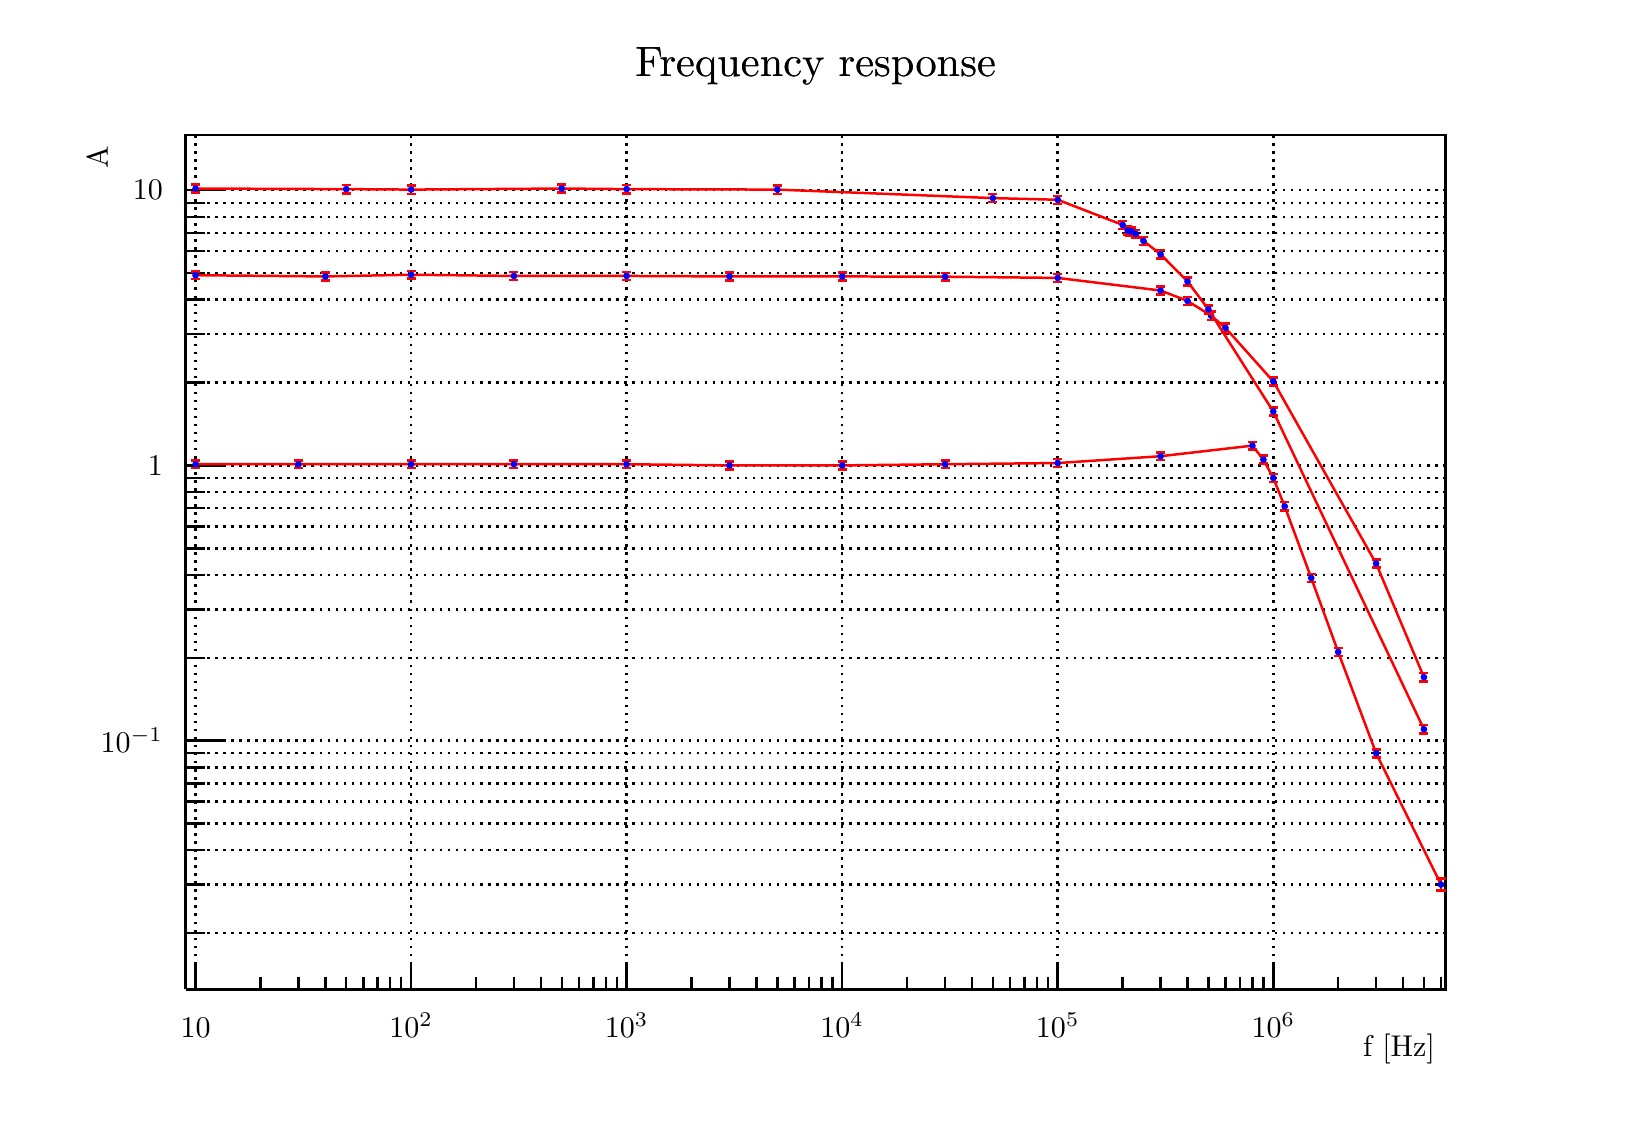
\begin{tikzpicture}
\pgfdeclareplotmark{cross} {
\pgfpathmoveto{\pgfpoint{-0.3\pgfplotmarksize}{\pgfplotmarksize}}
\pgfpathlineto{\pgfpoint{+0.3\pgfplotmarksize}{\pgfplotmarksize}}
\pgfpathlineto{\pgfpoint{+0.3\pgfplotmarksize}{0.3\pgfplotmarksize}}
\pgfpathlineto{\pgfpoint{+1\pgfplotmarksize}{0.3\pgfplotmarksize}}
\pgfpathlineto{\pgfpoint{+1\pgfplotmarksize}{-0.3\pgfplotmarksize}}
\pgfpathlineto{\pgfpoint{+0.3\pgfplotmarksize}{-0.3\pgfplotmarksize}}
\pgfpathlineto{\pgfpoint{+0.3\pgfplotmarksize}{-1.\pgfplotmarksize}}
\pgfpathlineto{\pgfpoint{-0.3\pgfplotmarksize}{-1.\pgfplotmarksize}}
\pgfpathlineto{\pgfpoint{-0.3\pgfplotmarksize}{-0.3\pgfplotmarksize}}
\pgfpathlineto{\pgfpoint{-1.\pgfplotmarksize}{-0.3\pgfplotmarksize}}
\pgfpathlineto{\pgfpoint{-1.\pgfplotmarksize}{0.3\pgfplotmarksize}}
\pgfpathlineto{\pgfpoint{-0.3\pgfplotmarksize}{0.3\pgfplotmarksize}}
\pgfpathclose
\pgfusepathqstroke
}
\pgfdeclareplotmark{cross*} {
\pgfpathmoveto{\pgfpoint{-0.3\pgfplotmarksize}{\pgfplotmarksize}}
\pgfpathlineto{\pgfpoint{+0.3\pgfplotmarksize}{\pgfplotmarksize}}
\pgfpathlineto{\pgfpoint{+0.3\pgfplotmarksize}{0.3\pgfplotmarksize}}
\pgfpathlineto{\pgfpoint{+1\pgfplotmarksize}{0.3\pgfplotmarksize}}
\pgfpathlineto{\pgfpoint{+1\pgfplotmarksize}{-0.3\pgfplotmarksize}}
\pgfpathlineto{\pgfpoint{+0.3\pgfplotmarksize}{-0.3\pgfplotmarksize}}
\pgfpathlineto{\pgfpoint{+0.3\pgfplotmarksize}{-1.\pgfplotmarksize}}
\pgfpathlineto{\pgfpoint{-0.3\pgfplotmarksize}{-1.\pgfplotmarksize}}
\pgfpathlineto{\pgfpoint{-0.3\pgfplotmarksize}{-0.3\pgfplotmarksize}}
\pgfpathlineto{\pgfpoint{-1.\pgfplotmarksize}{-0.3\pgfplotmarksize}}
\pgfpathlineto{\pgfpoint{-1.\pgfplotmarksize}{0.3\pgfplotmarksize}}
\pgfpathlineto{\pgfpoint{-0.3\pgfplotmarksize}{0.3\pgfplotmarksize}}
\pgfpathclose
\pgfusepathqfillstroke
}
\pgfdeclareplotmark{newstar} {
\pgfpathmoveto{\pgfqpoint{0pt}{\pgfplotmarksize}}
\pgfpathlineto{\pgfqpointpolar{44}{0.5\pgfplotmarksize}}
\pgfpathlineto{\pgfqpointpolar{18}{\pgfplotmarksize}}
\pgfpathlineto{\pgfqpointpolar{-20}{0.5\pgfplotmarksize}}
\pgfpathlineto{\pgfqpointpolar{-54}{\pgfplotmarksize}}
\pgfpathlineto{\pgfqpointpolar{-90}{0.5\pgfplotmarksize}}
\pgfpathlineto{\pgfqpointpolar{234}{\pgfplotmarksize}}
\pgfpathlineto{\pgfqpointpolar{198}{0.5\pgfplotmarksize}}
\pgfpathlineto{\pgfqpointpolar{162}{\pgfplotmarksize}}
\pgfpathlineto{\pgfqpointpolar{134}{0.5\pgfplotmarksize}}
\pgfpathclose
\pgfusepathqstroke
}
\pgfdeclareplotmark{newstar*} {
\pgfpathmoveto{\pgfqpoint{0pt}{\pgfplotmarksize}}
\pgfpathlineto{\pgfqpointpolar{44}{0.5\pgfplotmarksize}}
\pgfpathlineto{\pgfqpointpolar{18}{\pgfplotmarksize}}
\pgfpathlineto{\pgfqpointpolar{-20}{0.5\pgfplotmarksize}}
\pgfpathlineto{\pgfqpointpolar{-54}{\pgfplotmarksize}}
\pgfpathlineto{\pgfqpointpolar{-90}{0.5\pgfplotmarksize}}
\pgfpathlineto{\pgfqpointpolar{234}{\pgfplotmarksize}}
\pgfpathlineto{\pgfqpointpolar{198}{0.5\pgfplotmarksize}}
\pgfpathlineto{\pgfqpointpolar{162}{\pgfplotmarksize}}
\pgfpathlineto{\pgfqpointpolar{134}{0.5\pgfplotmarksize}}
\pgfpathclose
\pgfusepathqfillstroke
}
\definecolor{c}{rgb}{1,1,1};
\draw [color=c, fill=c] (0,0) rectangle (20,13.5632);
\draw [color=c, fill=c] (2,1.35632) rectangle (18,12.2069);
\definecolor{c}{rgb}{0,0,0};
\draw [c,line width=0.9] (2,1.35632) -- (2,12.2069) -- (18,12.2069) -- (18,1.35632) -- (2,1.35632);
\draw [c,line width=0.9] (2,1.35632) -- (18,1.35632);
\draw [c,dotted,line width=0.9] (2.12525,12.2069) -- (2.12525,1.35632);
\draw [c,dotted,line width=0.9] (4.86259,12.2069) -- (4.86259,1.35632);
\draw [c,dotted,line width=0.9] (7.59993,12.2069) -- (7.59993,1.35632);
\draw [c,dotted,line width=0.9] (10.3373,12.2069) -- (10.3373,1.35632);
\draw [c,dotted,line width=0.9] (13.0746,12.2069) -- (13.0746,1.35632);
\draw [c,dotted,line width=0.9] (15.8119,12.2069) -- (15.8119,1.35632);
\draw [c,line width=0.9] (2,1.35632) -- (2,12.2069);
\draw [c,dotted,line width=0.9] (18,2.07246) -- (2,2.07246);
\draw [c,dotted,line width=0.9] (18,2.68795) -- (2,2.68795);
\draw [c,dotted,line width=0.9] (18,3.12465) -- (2,3.12465);
\draw [c,dotted,line width=0.9] (18,3.46337) -- (2,3.46337);
\draw [c,dotted,line width=0.9] (18,3.74013) -- (2,3.74013);
\draw [c,dotted,line width=0.9] (18,3.97413) -- (2,3.97413);
\draw [c,dotted,line width=0.9] (18,4.17683) -- (2,4.17683);
\draw [c,dotted,line width=0.9] (18,4.35562) -- (2,4.35562);
\draw [c,dotted,line width=0.9] (18,4.51556) -- (2,4.51556);
\draw [c,dotted,line width=0.9] (18,5.56774) -- (2,5.56774);
\draw [c,dotted,line width=0.9] (18,6.18323) -- (2,6.18323);
\draw [c,dotted,line width=0.9] (18,6.61992) -- (2,6.61992);
\draw [c,dotted,line width=0.9] (18,6.95865) -- (2,6.95865);
\draw [c,dotted,line width=0.9] (18,7.23541) -- (2,7.23541);
\draw [c,dotted,line width=0.9] (18,7.46941) -- (2,7.46941);
\draw [c,dotted,line width=0.9] (18,7.67211) -- (2,7.67211);
\draw [c,dotted,line width=0.9] (18,7.8509) -- (2,7.8509);
\draw [c,dotted,line width=0.9] (18,8.01083) -- (2,8.01083);
\draw [c,dotted,line width=0.9] (18,9.06302) -- (2,9.06302);
\draw [c,dotted,line width=0.9] (18,9.67851) -- (2,9.67851);
\draw [c,dotted,line width=0.9] (18,10.1152) -- (2,10.1152);
\draw [c,dotted,line width=0.9] (18,10.4539) -- (2,10.4539);
\draw [c,dotted,line width=0.9] (18,10.7307) -- (2,10.7307);
\draw [c,dotted,line width=0.9] (18,10.9647) -- (2,10.9647);
\draw [c,dotted,line width=0.9] (18,11.1674) -- (2,11.1674);
\draw [c,dotted,line width=0.9] (18,11.3462) -- (2,11.3462);
\draw [c,dotted,line width=0.9] (18,11.5061) -- (2,11.5061);
\draw [c,line width=0.9] (2,1.35632) -- (18,1.35632);
\draw [anchor= east] (18,0.596782) node[scale=1.08496, color=c, rotate=0]{f [Hz]};
\draw [c,line width=0.9] (2.12525,1.68184) -- (2.12525,1.35632);
\draw [anchor=base] (2.12525,0.742586) node[scale=1.08496, color=c, rotate=0]{10};
\draw [c,line width=0.9] (2.94927,1.51908) -- (2.94927,1.35632);
\draw [c,line width=0.9] (3.43129,1.51908) -- (3.43129,1.35632);
\draw [c,line width=0.9] (3.77329,1.51908) -- (3.77329,1.35632);
\draw [c,line width=0.9] (4.03857,1.51908) -- (4.03857,1.35632);
\draw [c,line width=0.9] (4.25531,1.51908) -- (4.25531,1.35632);
\draw [c,line width=0.9] (4.43857,1.51908) -- (4.43857,1.35632);
\draw [c,line width=0.9] (4.59731,1.51908) -- (4.59731,1.35632);
\draw [c,line width=0.9] (4.73733,1.51908) -- (4.73733,1.35632);
\draw [c,line width=0.9] (4.86259,1.68184) -- (4.86259,1.35632);
\draw [anchor=base] (4.86259,0.742586) node[scale=1.08496, color=c, rotate=0]{$10^{2}$};
\draw [c,line width=0.9] (5.68661,1.51908) -- (5.68661,1.35632);
\draw [c,line width=0.9] (6.16863,1.51908) -- (6.16863,1.35632);
\draw [c,line width=0.9] (6.51063,1.51908) -- (6.51063,1.35632);
\draw [c,line width=0.9] (6.7759,1.51908) -- (6.7759,1.35632);
\draw [c,line width=0.9] (6.99265,1.51908) -- (6.99265,1.35632);
\draw [c,line width=0.9] (7.17591,1.51908) -- (7.17591,1.35632);
\draw [c,line width=0.9] (7.33465,1.51908) -- (7.33465,1.35632);
\draw [c,line width=0.9] (7.47467,1.51908) -- (7.47467,1.35632);
\draw [c,line width=0.9] (7.59993,1.68184) -- (7.59993,1.35632);
\draw [anchor=base] (7.59993,0.742586) node[scale=1.08496, color=c, rotate=0]{$10^{3}$};
\draw [c,line width=0.9] (8.42395,1.51908) -- (8.42395,1.35632);
\draw [c,line width=0.9] (8.90597,1.51908) -- (8.90597,1.35632);
\draw [c,line width=0.9] (9.24797,1.51908) -- (9.24797,1.35632);
\draw [c,line width=0.9] (9.51324,1.51908) -- (9.51324,1.35632);
\draw [c,line width=0.9] (9.72999,1.51908) -- (9.72999,1.35632);
\draw [c,line width=0.9] (9.91324,1.51908) -- (9.91324,1.35632);
\draw [c,line width=0.9] (10.072,1.51908) -- (10.072,1.35632);
\draw [c,line width=0.9] (10.212,1.51908) -- (10.212,1.35632);
\draw [c,line width=0.9] (10.3373,1.68184) -- (10.3373,1.35632);
\draw [anchor=base] (10.3373,0.742586) node[scale=1.08496, color=c, rotate=0]{$10^{4}$};
\draw [c,line width=0.9] (11.1613,1.51908) -- (11.1613,1.35632);
\draw [c,line width=0.9] (11.6433,1.51908) -- (11.6433,1.35632);
\draw [c,line width=0.9] (11.9853,1.51908) -- (11.9853,1.35632);
\draw [c,line width=0.9] (12.2506,1.51908) -- (12.2506,1.35632);
\draw [c,line width=0.9] (12.4673,1.51908) -- (12.4673,1.35632);
\draw [c,line width=0.9] (12.6506,1.51908) -- (12.6506,1.35632);
\draw [c,line width=0.9] (12.8093,1.51908) -- (12.8093,1.35632);
\draw [c,line width=0.9] (12.9493,1.51908) -- (12.9493,1.35632);
\draw [c,line width=0.9] (13.0746,1.68184) -- (13.0746,1.35632);
\draw [anchor=base] (13.0746,0.742586) node[scale=1.08496, color=c, rotate=0]{$10^{5}$};
\draw [c,line width=0.9] (13.8986,1.51908) -- (13.8986,1.35632);
\draw [c,line width=0.9] (14.3806,1.51908) -- (14.3806,1.35632);
\draw [c,line width=0.9] (14.7226,1.51908) -- (14.7226,1.35632);
\draw [c,line width=0.9] (14.9879,1.51908) -- (14.9879,1.35632);
\draw [c,line width=0.9] (15.2047,1.51908) -- (15.2047,1.35632);
\draw [c,line width=0.9] (15.3879,1.51908) -- (15.3879,1.35632);
\draw [c,line width=0.9] (15.5467,1.51908) -- (15.5467,1.35632);
\draw [c,line width=0.9] (15.6867,1.51908) -- (15.6867,1.35632);
\draw [c,line width=0.9] (15.8119,1.68184) -- (15.8119,1.35632);
\draw [anchor=base] (15.8119,0.742586) node[scale=1.08496, color=c, rotate=0]{$10^{6}$};
\draw [c,line width=0.9] (16.636,1.51908) -- (16.636,1.35632);
\draw [c,line width=0.9] (17.118,1.51908) -- (17.118,1.35632);
\draw [c,line width=0.9] (17.46,1.51908) -- (17.46,1.35632);
\draw [c,line width=0.9] (17.7253,1.51908) -- (17.7253,1.35632);
\draw [c,line width=0.9] (17.942,1.51908) -- (17.942,1.35632);
\draw [c,line width=0.9] (2,1.35632) -- (2,12.2069);
\draw [anchor= east] (0.88,12.2069) node[scale=1.08496, color=c, rotate=90]{A};
\draw [c,line width=0.9] (2.24,2.07246) -- (2,2.07246);
\draw [c,line width=0.9] (2.24,2.68795) -- (2,2.68795);
\draw [c,line width=0.9] (2.24,3.12465) -- (2,3.12465);
\draw [c,line width=0.9] (2.24,3.46337) -- (2,3.46337);
\draw [c,line width=0.9] (2.24,3.74013) -- (2,3.74013);
\draw [c,line width=0.9] (2.24,3.97413) -- (2,3.97413);
\draw [c,line width=0.9] (2.24,4.17683) -- (2,4.17683);
\draw [c,line width=0.9] (2.24,4.35562) -- (2,4.35562);
\draw [c,line width=0.9] (2.48,4.51556) -- (2,4.51556);
\draw [anchor= east] (1.844,4.51556) node[scale=1.08496, color=c, rotate=0]{$10^{-1}$};
\draw [c,line width=0.9] (2.24,5.56774) -- (2,5.56774);
\draw [c,line width=0.9] (2.24,6.18323) -- (2,6.18323);
\draw [c,line width=0.9] (2.24,6.61992) -- (2,6.61992);
\draw [c,line width=0.9] (2.24,6.95865) -- (2,6.95865);
\draw [c,line width=0.9] (2.24,7.23541) -- (2,7.23541);
\draw [c,line width=0.9] (2.24,7.46941) -- (2,7.46941);
\draw [c,line width=0.9] (2.24,7.67211) -- (2,7.67211);
\draw [c,line width=0.9] (2.24,7.8509) -- (2,7.8509);
\draw [c,line width=0.9] (2.48,8.01083) -- (2,8.01083);
\draw [anchor= east] (1.844,8.01083) node[scale=1.08496, color=c, rotate=0]{1};
\draw [c,line width=0.9] (2.24,9.06302) -- (2,9.06302);
\draw [c,line width=0.9] (2.24,9.67851) -- (2,9.67851);
\draw [c,line width=0.9] (2.24,10.1152) -- (2,10.1152);
\draw [c,line width=0.9] (2.24,10.4539) -- (2,10.4539);
\draw [c,line width=0.9] (2.24,10.7307) -- (2,10.7307);
\draw [c,line width=0.9] (2.24,10.9647) -- (2,10.9647);
\draw [c,line width=0.9] (2.24,11.1674) -- (2,11.1674);
\draw [c,line width=0.9] (2.24,11.3462) -- (2,11.3462);
\draw [c,line width=0.9] (2.48,11.5061) -- (2,11.5061);
\draw [anchor= east] (1.844,11.5061) node[scale=1.08496, color=c, rotate=0]{10};
\draw (10,13.0816) node[scale=1.5317, color=c, rotate=0]{Frequency response};
\definecolor{c}{rgb}{1,0,0};
\draw [c,line width=0.9] (2.12525,8.02594) -- (2.12525,8.07514);
\draw [c,line width=0.9] (2.06778,8.07514) -- (2.18272,8.07514);
\draw [c,line width=0.9] (2.12525,8.02594) -- (2.12525,7.97509);
\draw [c,line width=0.9] (2.06778,7.97509) -- (2.18272,7.97509);
\draw [c,line width=0.9] (3.4313,8.02594) -- (3.4313,8.07514);
\draw [c,line width=0.9] (3.37382,8.07514) -- (3.48877,8.07514);
\draw [c,line width=0.9] (3.4313,8.02594) -- (3.4313,7.97509);
\draw [c,line width=0.9] (3.37382,7.97509) -- (3.48877,7.97509);
\draw [c,line width=0.9] (4.86259,8.02594) -- (4.86259,8.07514);
\draw [c,line width=0.9] (4.80512,8.07514) -- (4.92006,8.07514);
\draw [c,line width=0.9] (4.86259,8.02594) -- (4.86259,7.97509);
\draw [c,line width=0.9] (4.80512,7.97509) -- (4.92006,7.97509);
\draw [c,line width=0.9] (6.16863,8.02594) -- (6.16863,8.07514);
\draw [c,line width=0.9] (6.11116,8.07514) -- (6.2261,8.07514);
\draw [c,line width=0.9] (6.16863,8.02594) -- (6.16863,7.97509);
\draw [c,line width=0.9] (6.11116,7.97509) -- (6.2261,7.97509);
\draw [c,line width=0.9] (7.59993,8.02594) -- (7.59993,8.07514);
\draw [c,line width=0.9] (7.54246,8.07514) -- (7.6574,8.07514);
\draw [c,line width=0.9] (7.59993,8.02594) -- (7.59993,7.97509);
\draw [c,line width=0.9] (7.54246,7.97509) -- (7.6574,7.97509);
\draw [c,line width=0.9] (8.90597,8.01083) -- (8.90597,8.0601);
\draw [c,line width=0.9] (8.8485,8.0601) -- (8.96344,8.0601);
\draw [c,line width=0.9] (8.90597,8.01083) -- (8.90597,7.95992);
\draw [c,line width=0.9] (8.8485,7.95992) -- (8.96344,7.95992);
\draw [c,line width=0.9] (10.3373,8.01083) -- (10.3373,8.0601);
\draw [c,line width=0.9] (10.2798,8.0601) -- (10.3947,8.0601);
\draw [c,line width=0.9] (10.3373,8.01083) -- (10.3373,7.95992);
\draw [c,line width=0.9] (10.2798,7.95992) -- (10.3947,7.95992);
\draw [c,line width=0.9] (11.6433,8.02594) -- (11.6433,8.07514);
\draw [c,line width=0.9] (11.5858,8.07514) -- (11.7008,8.07514);
\draw [c,line width=0.9] (11.6433,8.02594) -- (11.6433,7.97509);
\draw [c,line width=0.9] (11.5858,7.97509) -- (11.7008,7.97509);
\draw [c,line width=0.9] (13.0746,8.04089) -- (13.0746,8.09003);
\draw [c,line width=0.9] (13.0171,8.09003) -- (13.1321,8.09003);
\draw [c,line width=0.9] (13.0746,8.04089) -- (13.0746,7.99011);
\draw [c,line width=0.9] (13.0171,7.99011) -- (13.1321,7.99011);
\draw [c,line width=0.9] (14.3806,8.12766) -- (14.3806,8.17646);
\draw [c,line width=0.9] (14.3232,8.17646) -- (14.4381,8.17646);
\draw [c,line width=0.9] (14.3806,8.12766) -- (14.3806,8.07724);
\draw [c,line width=0.9] (14.3232,8.07724) -- (14.4381,8.07724);
\draw [c,line width=0.9] (15.5467,8.26208) -- (15.5467,8.31043);
\draw [c,line width=0.9] (15.4892,8.31043) -- (15.6041,8.31043);
\draw [c,line width=0.9] (15.5467,8.26208) -- (15.5467,8.21214);
\draw [c,line width=0.9] (15.4892,8.21214) -- (15.6041,8.21214);
\draw [c,line width=0.9] (15.6867,8.0849) -- (15.6867,8.13386);
\draw [c,line width=0.9] (15.6292,8.13386) -- (15.7442,8.13386);
\draw [c,line width=0.9] (15.6867,8.0849) -- (15.6867,8.0343);
\draw [c,line width=0.9] (15.6292,8.0343) -- (15.7442,8.0343);
\draw [c,line width=0.9] (15.8119,7.8509) -- (15.8119,7.90091);
\draw [c,line width=0.9] (15.7545,7.90091) -- (15.8694,7.90091);
\draw [c,line width=0.9] (15.8119,7.8509) -- (15.8119,7.79919);
\draw [c,line width=0.9] (15.7545,7.79919) -- (15.8694,7.79919);
\draw [c,line width=0.9] (15.9572,7.49094) -- (15.9572,7.54326);
\draw [c,line width=0.9] (15.8998,7.54326) -- (16.0147,7.54326);
\draw [c,line width=0.9] (15.9572,7.49094) -- (15.9572,7.43675);
\draw [c,line width=0.9] (15.8998,7.43675) -- (16.0147,7.43675);
\draw [c,line width=0.9] (16.294,6.58149) -- (16.294,6.63277);
\draw [c,line width=0.9] (16.2365,6.63277) -- (16.3514,6.63277);
\draw [c,line width=0.9] (16.294,6.58149) -- (16.294,6.52841);
\draw [c,line width=0.9] (16.2365,6.52841) -- (16.3514,6.52841);
\draw [c,line width=0.9] (16.636,5.6418) -- (16.636,5.69238);
\draw [c,line width=0.9] (16.5785,5.69238) -- (16.6934,5.69238);
\draw [c,line width=0.9] (16.636,5.6418) -- (16.636,5.58948);
\draw [c,line width=0.9] (16.5785,5.58948) -- (16.6934,5.58948);
\draw [c,line width=0.9] (17.118,4.35562) -- (17.118,4.40563);
\draw [c,line width=0.9] (17.0605,4.40563) -- (17.1754,4.40563);
\draw [c,line width=0.9] (17.118,4.35562) -- (17.118,4.30391);
\draw [c,line width=0.9] (17.0605,4.30391) -- (17.1754,4.30391);
\draw [c,line width=0.9] (17.942,2.68795) -- (17.942,2.76264);
\draw [c,line width=0.9] (17.8845,2.76264) -- (18,2.76264);
\draw [c,line width=0.9] (17.942,2.68795) -- (17.942,2.60939);
\draw [c,line width=0.9] (17.8845,2.60939) -- (18,2.60939);
\draw [c,line width=0.9] (2.12525,8.02594) -- (3.4313,8.02594) -- (4.86259,8.02594) -- (6.16863,8.02594) -- (7.59993,8.02594) -- (8.90597,8.01083) -- (10.3373,8.01083) -- (11.6433,8.02594) -- (13.0746,8.04089) -- (14.3806,8.12766) --
 (15.5467,8.26208) -- (15.6867,8.0849) -- (15.8119,7.8509) -- (15.9572,7.49094) -- (16.294,6.58149) -- (16.636,5.6418) -- (17.118,4.35562) -- (17.942,2.68795);
\definecolor{c}{rgb}{0,0,1};
\foreach \P in {(2.12525,8.02594), (3.4313,8.02594), (4.86259,8.02594), (6.16863,8.02594), (7.59993,8.02594), (8.90597,8.01083), (10.3373,8.01083), (11.6433,8.02594), (13.0746,8.04089), (14.3806,8.12766), (15.5467,8.26208), (15.6867,8.0849),
 (15.8119,7.8509), (15.9572,7.49094), (16.294,6.58149), (16.636,5.6418), (17.118,4.35562), (17.942,2.68795)}{\draw[mark options={color=c,fill=c},mark size=1.681682pt,mark=*,mark size=1pt] plot coordinates {\P};}
\definecolor{c}{rgb}{1,0,0};
\draw [c,line width=0.9] (2.12525,10.4264) -- (2.12525,10.4757);
\draw [c,line width=0.9] (2.06778,10.4757) -- (2.18272,10.4757);
\draw [c,line width=0.9] (2.12525,10.4264) -- (2.12525,10.3753);
\draw [c,line width=0.9] (2.06778,10.3753) -- (2.18272,10.3753);
\draw [c,line width=0.9] (3.77329,10.4108) -- (3.77329,10.4603);
\draw [c,line width=0.9] (3.71582,10.4603) -- (3.83077,10.4603);
\draw [c,line width=0.9] (3.77329,10.4108) -- (3.77329,10.3597);
\draw [c,line width=0.9] (3.71582,10.3597) -- (3.83077,10.3597);
\draw [c,line width=0.9] (4.86259,10.4325) -- (4.86259,10.4819);
\draw [c,line width=0.9] (4.80512,10.4819) -- (4.92006,10.4819);
\draw [c,line width=0.9] (4.86259,10.4325) -- (4.86259,10.3815);
\draw [c,line width=0.9] (4.80512,10.3815) -- (4.92006,10.3815);
\draw [c,line width=0.9] (6.16863,10.4171) -- (6.16863,10.4665);
\draw [c,line width=0.9] (6.11116,10.4665) -- (6.2261,10.4665);
\draw [c,line width=0.9] (6.16863,10.4171) -- (6.16863,10.366);
\draw [c,line width=0.9] (6.11116,10.366) -- (6.2261,10.366);
\draw [c,line width=0.9] (7.59993,10.4171) -- (7.59993,10.4665);
\draw [c,line width=0.9] (7.54246,10.4665) -- (7.6574,10.4665);
\draw [c,line width=0.9] (7.59993,10.4171) -- (7.59993,10.366);
\draw [c,line width=0.9] (7.54246,10.366) -- (7.6574,10.366);
\draw [c,line width=0.9] (8.90597,10.4108) -- (8.90597,10.4603);
\draw [c,line width=0.9] (8.8485,10.4603) -- (8.96344,10.4603);
\draw [c,line width=0.9] (8.90597,10.4108) -- (8.90597,10.3597);
\draw [c,line width=0.9] (8.8485,10.3597) -- (8.96344,10.3597);
\draw [c,line width=0.9] (10.3373,10.4108) -- (10.3373,10.4603);
\draw [c,line width=0.9] (10.2798,10.4603) -- (10.3947,10.4603);
\draw [c,line width=0.9] (10.3373,10.4108) -- (10.3373,10.3597);
\draw [c,line width=0.9] (10.2798,10.3597) -- (10.3947,10.3597);
\draw [c,line width=0.9] (11.6433,10.4077) -- (11.6433,10.4572);
\draw [c,line width=0.9] (11.5858,10.4572) -- (11.7008,10.4572);
\draw [c,line width=0.9] (11.6433,10.4077) -- (11.6433,10.3566);
\draw [c,line width=0.9] (11.5858,10.3566) -- (11.7008,10.3566);
\draw [c,line width=0.9] (13.0746,10.392) -- (13.0746,10.4415);
\draw [c,line width=0.9] (13.0171,10.4415) -- (13.1321,10.4415);
\draw [c,line width=0.9] (13.0746,10.392) -- (13.0746,10.3408);
\draw [c,line width=0.9] (13.0171,10.3408) -- (13.1321,10.3408);
\draw [c,line width=0.9] (14.3806,10.232) -- (14.3806,10.2824);
\draw [c,line width=0.9] (14.3232,10.2824) -- (14.4381,10.2824);
\draw [c,line width=0.9] (14.3806,10.232) -- (14.3806,10.18);
\draw [c,line width=0.9] (14.3232,10.18) -- (14.4381,10.18);
\draw [c,line width=0.9] (14.7226,10.0999) -- (14.7226,10.1511);
\draw [c,line width=0.9] (14.6652,10.1511) -- (14.7801,10.1511);
\draw [c,line width=0.9] (14.7226,10.0999) -- (14.7226,10.047);
\draw [c,line width=0.9] (14.6652,10.047) -- (14.7801,10.047);
\draw [c,line width=0.9] (15.0231,9.9125) -- (15.0231,9.96499);
\draw [c,line width=0.9] (14.9656,9.96499) -- (15.0805,9.96499);
\draw [c,line width=0.9] (15.0231,9.9125) -- (15.0231,9.85813);
\draw [c,line width=0.9] (14.9656,9.85813) -- (15.0805,9.85813);
\draw [c,line width=0.9] (15.2047,9.75738) -- (15.2047,9.81124);
\draw [c,line width=0.9] (15.1472,9.81124) -- (15.2621,9.81124);
\draw [c,line width=0.9] (15.2047,9.75738) -- (15.2047,9.70154);
\draw [c,line width=0.9] (15.1472,9.70154) -- (15.2621,9.70154);
\draw [c,line width=0.9] (15.8119,9.07812) -- (15.8119,9.12906);
\draw [c,line width=0.9] (15.7545,9.12906) -- (15.8694,9.12906);
\draw [c,line width=0.9] (15.8119,9.07812) -- (15.8119,9.02542);
\draw [c,line width=0.9] (15.7545,9.02542) -- (15.8694,9.02542);
\draw [c,line width=0.9] (17.118,6.7646) -- (17.118,6.81479);
\draw [c,line width=0.9] (17.0605,6.81479) -- (17.1754,6.81479);
\draw [c,line width=0.9] (17.118,6.7646) -- (17.118,6.7127);
\draw [c,line width=0.9] (17.0605,6.7127) -- (17.1754,6.7127);
\draw [c,line width=0.9] (17.7253,5.32104) -- (17.7253,5.37152);
\draw [c,line width=0.9] (17.6678,5.37152) -- (17.7827,5.37152);
\draw [c,line width=0.9] (17.7253,5.32104) -- (17.7253,5.26882);
\draw [c,line width=0.9] (17.6678,5.26882) -- (17.7827,5.26882);
\draw [c,line width=0.9] (2.12525,10.4264) -- (3.77329,10.4108) -- (4.86259,10.4325) -- (6.16863,10.4171) -- (7.59993,10.4171) -- (8.90597,10.4108) -- (10.3373,10.4108) -- (11.6433,10.4077) -- (13.0746,10.392) -- (14.3806,10.232) -- (14.7226,10.0999)
 -- (15.0231,9.9125) -- (15.2047,9.75738) -- (15.8119,9.07812) -- (17.118,6.7646) -- (17.7253,5.32104);
\definecolor{c}{rgb}{0,0,1};
\foreach \P in {(2.12525,10.4264), (3.77329,10.4108), (4.86259,10.4325), (6.16863,10.4171), (7.59993,10.4171), (8.90597,10.4108), (10.3373,10.4108), (11.6433,10.4077), (13.0746,10.392), (14.3806,10.232), (14.7226,10.0999), (15.0231,9.9125),
 (15.2047,9.75738), (15.8119,9.07812), (17.118,6.7646), (17.7253,5.32104)}{\draw[mark options={color=c,fill=c},mark size=1.681682pt,mark=*,mark size=1pt] plot coordinates {\P};}
\definecolor{c}{rgb}{1,0,0};
\draw [c,line width=0.9] (2.12525,11.5272) -- (2.12525,11.5781);
\draw [c,line width=0.9] (2.06778,11.5781) -- (2.18272,11.5781);
\draw [c,line width=0.9] (2.12525,11.5272) -- (2.12525,11.4746);
\draw [c,line width=0.9] (2.06778,11.4746) -- (2.18272,11.4746);
\draw [c,line width=0.9] (4.03857,11.5197) -- (4.03857,11.5707);
\draw [c,line width=0.9] (3.9811,11.5707) -- (4.09604,11.5707);
\draw [c,line width=0.9] (4.03857,11.5197) -- (4.03857,11.467);
\draw [c,line width=0.9] (3.9811,11.467) -- (4.09604,11.467);
\draw [c,line width=0.9] (4.86259,11.5137) -- (4.86259,11.5647);
\draw [c,line width=0.9] (4.80512,11.5647) -- (4.92006,11.5647);
\draw [c,line width=0.9] (4.86259,11.5137) -- (4.86259,11.4609);
\draw [c,line width=0.9] (4.80512,11.4609) -- (4.92006,11.4609);
\draw [c,line width=0.9] (6.77591,11.5272) -- (6.77591,11.5781);
\draw [c,line width=0.9] (6.71843,11.5781) -- (6.83338,11.5781);
\draw [c,line width=0.9] (6.77591,11.5272) -- (6.77591,11.4746);
\draw [c,line width=0.9] (6.71843,11.4746) -- (6.83338,11.4746);
\draw [c,line width=0.9] (7.59993,11.5197) -- (7.59993,11.5707);
\draw [c,line width=0.9] (7.54246,11.5707) -- (7.6574,11.5707);
\draw [c,line width=0.9] (7.59993,11.5197) -- (7.59993,11.467);
\draw [c,line width=0.9] (7.54246,11.467) -- (7.6574,11.467);
\draw [c,line width=0.9] (9.51324,11.5137) -- (9.51324,11.5647);
\draw [c,line width=0.9] (9.45577,11.5647) -- (9.57071,11.5647);
\draw [c,line width=0.9] (9.51324,11.5137) -- (9.51324,11.4609);
\draw [c,line width=0.9] (9.45577,11.4609) -- (9.57071,11.4609);
\draw [c,line width=0.9] (12.2506,11.4057) -- (12.2506,11.4554);
\draw [c,line width=0.9] (12.1931,11.4554) -- (12.3081,11.4554);
\draw [c,line width=0.9] (12.2506,11.4057) -- (12.2506,11.3543);
\draw [c,line width=0.9] (12.1931,11.3543) -- (12.3081,11.3543);
\draw [c,line width=0.9] (13.0746,11.3845) -- (13.0746,11.4343);
\draw [c,line width=0.9] (13.0171,11.4343) -- (13.1321,11.4343);
\draw [c,line width=0.9] (13.0746,11.3845) -- (13.0746,11.333);
\draw [c,line width=0.9] (13.0171,11.333) -- (13.1321,11.333);
\draw [c,line width=0.9] (13.8986,11.0654) -- (13.8986,11.1171);
\draw [c,line width=0.9] (13.8411,11.1171) -- (13.9561,11.1171);
\draw [c,line width=0.9] (13.8986,11.0654) -- (13.8986,11.0118);
\draw [c,line width=0.9] (13.8411,11.0118) -- (13.9561,11.0118);
\draw [c,line width=0.9] (13.9623,10.9947) -- (13.9623,11.0443);
\draw [c,line width=0.9] (13.9048,11.0443) -- (14.0197,11.0443);
\draw [c,line width=0.9] (13.9623,10.9947) -- (13.9623,10.9435);
\draw [c,line width=0.9] (13.9048,10.9435) -- (14.0197,10.9435);
\draw [c,line width=0.9] (13.9846,10.9841) -- (13.9846,11.0337);
\draw [c,line width=0.9] (13.9271,11.0337) -- (14.0421,11.0337);
\draw [c,line width=0.9] (13.9846,10.9841) -- (13.9846,10.9328);
\draw [c,line width=0.9] (13.9271,10.9328) -- (14.0421,10.9328);
\draw [c,line width=0.9] (14.0119,10.9841) -- (14.0119,11.0337);
\draw [c,line width=0.9] (13.9545,11.0337) -- (14.0694,11.0337);
\draw [c,line width=0.9] (14.0119,10.9841) -- (14.0119,10.9328);
\draw [c,line width=0.9] (13.9545,10.9328) -- (14.0694,10.9328);
\draw [c,line width=0.9] (14.0648,10.9516) -- (14.0648,11.0014);
\draw [c,line width=0.9] (14.0073,11.0014) -- (14.1222,11.0014);
\draw [c,line width=0.9] (14.0648,10.9516) -- (14.0648,10.9001);
\draw [c,line width=0.9] (14.0073,10.9001) -- (14.1222,10.9001);
\draw [c,line width=0.9] (14.1639,10.8615) -- (14.1639,10.9118);
\draw [c,line width=0.9] (14.1064,10.9118) -- (14.2214,10.9118);
\draw [c,line width=0.9] (14.1639,10.8615) -- (14.1639,10.8095);
\draw [c,line width=0.9] (14.1064,10.8095) -- (14.2214,10.8095);
\draw [c,line width=0.9] (14.3806,10.6923) -- (14.3806,10.7435);
\draw [c,line width=0.9] (14.3232,10.7435) -- (14.4381,10.7435);
\draw [c,line width=0.9] (14.3806,10.6923) -- (14.3806,10.6392);
\draw [c,line width=0.9] (14.3232,10.6392) -- (14.4381,10.6392);
\draw [c,line width=0.9] (14.7226,10.347) -- (14.7226,10.3968);
\draw [c,line width=0.9] (14.6652,10.3968) -- (14.7801,10.3968);
\draw [c,line width=0.9] (14.7226,10.347) -- (14.7226,10.2956);
\draw [c,line width=0.9] (14.6652,10.2956) -- (14.7801,10.2956);
\draw [c,line width=0.9] (14.9879,9.99275) -- (14.9879,10.0446);
\draw [c,line width=0.9] (14.9304,10.0446) -- (15.0454,10.0446);
\draw [c,line width=0.9] (14.9879,9.99275) -- (14.9879,9.93904);
\draw [c,line width=0.9] (14.9304,9.93904) -- (15.0454,9.93904);
\draw [c,line width=0.9] (15.8119,8.69556) -- (15.8119,8.74678);
\draw [c,line width=0.9] (15.7545,8.74678) -- (15.8694,8.74678);
\draw [c,line width=0.9] (15.8119,8.69556) -- (15.8119,8.64255);
\draw [c,line width=0.9] (15.7545,8.64255) -- (15.8694,8.64255);
\draw [c,line width=0.9] (17.7253,4.66023) -- (17.7253,4.71218);
\draw [c,line width=0.9] (17.6678,4.71218) -- (17.7827,4.71218);
\draw [c,line width=0.9] (17.7253,4.66023) -- (17.7253,4.60645);
\draw [c,line width=0.9] (17.6678,4.60645) -- (17.7827,4.60645);
\draw [c,line width=0.9] (2.12525,11.5272) -- (4.03857,11.5197) -- (4.86259,11.5137) -- (6.77591,11.5272) -- (7.59993,11.5197) -- (9.51324,11.5137) -- (12.2506,11.4057) -- (13.0746,11.3845) -- (13.8986,11.0654) -- (13.9623,10.9947) --
 (13.9846,10.9841) -- (14.0119,10.9841) -- (14.0648,10.9516) -- (14.1639,10.8615) -- (14.3806,10.6923) -- (14.7226,10.347) -- (14.9879,9.99275) -- (15.8119,8.69556) -- (17.7253,4.66023);
\definecolor{c}{rgb}{0,0,1};
\foreach \P in {(2.12525,11.5272), (4.03857,11.5197), (4.86259,11.5137), (6.77591,11.5272), (7.59993,11.5197), (9.51324,11.5137), (12.2506,11.4057), (13.0746,11.3845), (13.8986,11.0654), (13.9623,10.9947), (13.9846,10.9841), (14.0119,10.9841),
 (14.0648,10.9516), (14.1639,10.8615), (14.3806,10.6923), (14.7226,10.347), (14.9879,9.99275), (15.8119,8.69556), (17.7253,4.66023)}{\draw[mark options={color=c,fill=c},mark size=1.681682pt,mark=*,mark size=1pt] plot coordinates {\P};}
\definecolor{c}{rgb}{0,0,0};
\draw (10,13.0816) node[scale=1.5317, color=c, rotate=0]{Frequency response};
\end{tikzpicture}
 
 \caption{Risposta in frequenza di un amplificatore non invertente a varie amplificazioni} 
 \label{gr:amp_noninv_all.tex} 
\end{grafico}
%Discutere come si comporta la variabile GBP 
%IL GBP FA SCHIFO


